\chapter{稳恒电流}
\section{教学要求}
这一章是电学部分的重点章,本章讲授的直流电路基本
知识,有较大的实用价值,是学习电工和电子技术的基础,对
日常生活和生产中使用电器也很有用。

教材注意了联系前章学过的电场知识,注意了联系实际。
在讲电流的产生、电功、电路中的电势降落等知识时,注意用
前章学过的电场、电势能、电势等知识给予说明,以加深学生
的理解。在讲串联和并联电路、电路的分析和计算、闭合电路
的欧姆定律等知识时,注意它们的实际应用,在培养能力方
面,注意教给学生分析解决电路问题的方法。

全章教材共十四节,可以划分为五个单元,第一节到第
三节为第一单元,讲述直流电路的一些基本概念和规律。第
四节和第五节为第二单元,从功和能的观点研究电路中的电
能转化。第六节到第九节为第三单元,讲述串联电路和并联
电路,以及简单的混联电路。第十节到第十二节为第四单元,
讲述闭合电路的欧姆定律及其应用。第十三节和第十四节为
第五单元,讲述测量电阻的方法。

部分电路欧姆定律和闭合电路欧姆定律是电学中最基本
的规律之一,它们不仅是解决直流电路有关计算的依据,而且
对学习交流电路有重要作用。所以,欧姆定律是全章的中心
和贯穿全章教材的主线。电流、电压、电动势和电阻是稳恒电
流的几个基本理量,欧姆定律正反映了这些量之间的相互
关系;电功、电功率、焦耳定律都和欧姆定律有着密切联系,研
究了电能与其他形式能的转化,有重要的实际意义;串联电路
和并联电路是电路连接的基本形式,掌握串、并联电路的基本
特点,是应用欧姆定律进行电路计算的关键,这些知识都很
重要,是研究直流电路的基础和工具,电池组在生活、生产和
实验中都常用。学生应该知道并联电池组和串联电池组的
特点,并能根据实际需要选用和组成电池组。电阻的测量在
电学实验、业余无线电活动以及生活、生产中经常遇到。教材
讲解电阻的测量主要是综合运用本章学过的知识,以提高学
生运用知识的能力。值得说明的是,电动势的概念尽管重要,
但由于这个概念比较复杂,限于学生的知识水平,中学阶段很
难讲清楚,不要求涉及电源内部的情况和电动势是怎样产
生的。

这一章的教学要求是:
\begin{enumerate}
\item 了解电流的产生条件,理解电流强度的概念,理解电
阻和电阻率的概念,掌握电阻定律。巩固掌握欧姆定律。
\item 理解电功和电功率的概念,掌握电功和电功率的公
式,掌握焦耳定律,了解电功和电热的关系
\item 巩固掌握串联电路和并联电路的特点,会分析、解决
直流电路中的混联问题。
\item 了解电动势的概念,巩固掌握闭合电路的欧姆定律。
掌握串联电池组及并联电池组的计算和应用,了解混联电池
组的应用。
\item 理解用伏安法和欧姆表法测电阻的原理。
\end{enumerate}

\section{教学建议}
本章教学的重点是闭合电路欧姆定律,难点是电动势概
念以及电动的几个公式的意义和运用条件。

由于全章教材内容具有鲜明的实践性,教学中应当加强
演示实验和学生实验,培养学生的实验能力。要特别注意教
给学生分析问题的思路和方法,培养他们的思维能力及应用
物理规律解决实际问题的能力。


\subsection{第一单元}
这一单元主要复习初中教材的电流强度、电阻、以及欧姆
定律,并在复习的基础上应用电场理论适当予以深化、提高。
同时补充学习电阻定律、电阻率等新知识。初中受学生知识
水平和思维能力发展的限制,只能从生活经验及实验事实出
发讲得比较简单,考虑到不学好这些概念、规律,很难进一步
学好其他电学知识,而在学过电场知识以后又可能讲得更深
入一些,因此教材仍把它们作为重要内容认真讲述。教学中
切不可因为学生已有一定的基础而掉以轻心,既要重视突出
知识的要点,又应当针对学生容易出错的问题,采用适当的教
学方法予以强调。

\subsubsection{电流}

电流产生的条件可按教材讲述的层次,利用课
本图7.1和图7.2, 逐步引导学生认识:
\begin{enumerate}
\item 形成电流
的条件是既要有能自由移动的电荷-自由电荷,又必须在
导体中建立电场.    \item 由于导体内存在自由电荷,所以导体中
存在持续电流的条件是保持导体两端有电势差。电源的作用
正是为了保持电路两端的电势差,使电路中存在持续电流。
\item 在学完稳恒电流与直流电的区别后应明确:要得到大小、
方向都不随时间变化的稳恒电流,导体两端的电势差必须保
持恒定。
\end{enumerate}

教材指出“自由电子除了做无规则的热运动外,还要在电
场力的作用下做定向移动,”对这段叙述,学生往往缺乏清晰
的认识,应当指出,自由电子作定向运动时,其无规则热运动
并未消失。它们一方面继续作无规则热运动,另一方面又沿
某一方向定向运动,即在无规则热运动速度的基础上叠加了
一个定向移动速度。为了避免学生从生活经验出发认为自由
电子定向移动速率非常大的错误,可以把第八章中关于自由
电子热运动的平均速率,定向移动速率和电场传播速率的数
量级分别为105$\ms$、$10^{-5}\ms$,$3\x10^8\ms$提前介绍.强
调电流传导速率实际上是电场传播速率,而不是自由电子定
向移动速率。

在讲解电流强度的概念及电流方向时,可以提出一些问
题让学生讨论,如:
\begin{enumerate}
\item 当通过不同横截面积的几根导线的电
流强度相等时,在相同时间内通过各导线横截面的电量跟截
面积大小有无关系?为什么?    
\item 为什么说导体中电流的方向总是从电势高的一端流向电势低的一端?
\item 电解液中电流强
度的大小和方向怎样确定?通过讨论加深学生对这部分知识
的理解,澄清一些模糊认识。
\end{enumerate}


\subsubsection{欧姆定律}

电阻是电路中的三个基本物理量之一,正
确理解电阻的物理意义对理解和掌握欧姆定律有重要作用。
因此,教材首先对电阻的概念作了认真的剖析。$R=U/I$
是电
阻的定义式,表明了一种量度电阻的方法。但学生在学习中
往往出现以下错误,如“电阻跟电压成正比,跟电流强度成反
比。”“既然电阻是表示导体对电流的阻碍作用的物理量,所以
导体中没有电流时导体就不存在电阻。”教学中应当有针对性
地将这些问题提出来讨论,以阐明$R=U/I$
的物理意义,纠正学
生的错误认识。要强调对金属和电解液电阻R是一个只与导
体本身有关的量。当导体的材料、粗细、长度、温度等因素一
定后,导体的电阻就确定了。电压和电流变化了,它们的比值$U/I$
即$R$是不会变的。同时应当指出,不管有无电流通过导体,
反映导体对电流阻碍作用大小的电阻$R$是客观存在的,只不
过当有电流通过导体时,这个作用才具体表现出来。

在进行欧姆定律$I=U/R$
的教学时,应通过具体题目的分
析,反复强调公式中的$U$、$I$、$R$是表示同一段电路的三个物
理量,决不能把属于不同电路的$U$、$I$、$R$值代入公式计算。

伏-安特性曲线是说明物质导电特性常用的一种表示方
法,在电工学和无线电电子学中有着广泛应用,要让学生对
此有所了解。应引导学生认识金属导体和电解液的伏-安特
性曲线是通过坐标原点的一条直线,具有这种性质的电阻叫
线性电阻,直线的斜率等于导体电阻的倒数。因此,通过比
较直线斜率的大小可以判断电阻的大小,但是有的导体和元
件,如热敏电阻、晶体二极管、真空二极管等的伏-安特性曲
线都不是直线而是特殊形状的曲线。这些导体和元件的电阻
就不是线性电阻而是非线性电阻了。它们的电阻$R$不是一个
常量,其大小与电压、电流的值有关。所以,它们不遵从欧
姆定律。

从线性电阻和非线性电阻的伏-安特性曲线的分析,我
们可以看出,尽管欧姆定律$I=U/R$
和电阻的定义式$R=U/I$
从数学形式上并无本质不同,但是物理意义却有区别。线性
电阻遵从欧姆定律,非线性电阻不遵从欧姆定律,然而,无论
线性还是非线性电阻都可以用$R=U/I$
来定义。这个问题只要
点到就行,不必展开讲解。

\subsubsection{电阻定律和电阻率}

电阻定律是一个实验定律.由
于在初中只作过定性实验,为了增加学生的感性认识,熟悉运
用实验总结物理规律的研究方法,在教学中有必要通过定量
实验得出电阻定律$R=\rho\ell/S$.
并且说明电阻定律不是对所有
导体都适用的电阻定义式,它适用于粗细均匀的金属导体及
浓度均匀一致的电解液。它定量揭示了这类导体的电阻由自
身的哪些物理条件决定,也反映了这类导体的电阻大小跟加
在导体两端的电压和通过的电流强度无关。

材料的电阻率$\rho$是描述材料导电性好坏的一个物理量,
可按教材安排的顺序分以下几步讲解.
\begin{enumerate}
\item 从分析电阻定律$R=\rho\ell/S$
中比例系数$\rho$的意义入手,讲清电阻率的意义.
\item 
强调指出电阻率与导体的大小、形状无关,仅取决于导体材料
的性质和导体所处的条件(如温度).公式$\rho=RS/\ell$
表示材料
的电阻率在数值上等于这种材料制成的长1m,横截面积
$1{\rm m^2}$的导体的电阻.
\item 说明在国际单位制中电阻率单位为
什么是欧姆·米。
\item 引导学生讨论电阻和电阻率有什么区
别,使他们认识到电阻率反映物质对电流阻碍作用的特性,
电阻则反映物体对电流阻碍作用的特性,因此,前者仅与物
质种类有关,后者却不但与构成物体的物质种类有关还与物
体的长度、横截面积有关。教材练习二第3题有助于学生理
解这个问题,可安排课堂讨论.
\item 指导学生阅读教材180页
的表列数值,使他们对常用金属的导电性能强弱有一个清楚
的认识。
\end{enumerate}

各种物质的电阻率都和温度有关,因此,各种导体的电阻
也都随温度变化。实验表明,所有纯金属的电阻率都随温度
升高而增大。为了加强教学的直观性,可以增加如下一个演
示实验:把一个废白炽灯泡的玻璃外壳小心去掉,取其内部一
段几厘米长的钨丝接在灯芯的灯丝支架上,与一个1.5伏电
源,一个安培表接成串联电路,测出电流强度,然后用酒精
灯把灯丝烧红,将看到电流强度明显减小。从而定性说明温
度越高,金属电阻率越大。精确实验证明,当温度变化范围不
大时,电阻率跟温度近似有如下线性关系$\rho=\rho_0(1+\alpha t)$. 式
中$\rho$和$\rho_0$分别是温度为$t$和$0^{\circ}{\rm C}$时材料的电阻率,$\alpha$为材料的
温度系数.多数纯金属的$\alpha$值近似等于$4\x10^{-3}/$度.对电
阻率跟温度的这个定量关系式,一般不宜在课堂上讲授,如:
果教师认为有必要介绍,也只需让学生知道就行,不要作过多
的阐述。但是,应当向学生指出:今后在涉及电阻值的计算
时,为使问题简化,如果没有特殊要求,我们通常不考虑温度
对电阻率的影响。

关于超导体的讲授,可引用后面参考资料提供的材料,适
当充实教学内容,以开阔学生眼界,激发他们进行科学探索的
志趣。

\subsection{第二单元}
这一单元仍属复习提高性质,目的在于使学生从电场力
做功和电势能变化的角度加深对电流做功的理解,搞清楚电
路中的能量转化关系。

\subsubsection{电功和电功率}

根据教材的逻辑顺序,从复习电场力
移动电荷做功$W=qU$结合电流强度的定义式$I=q/t$
推导出
电流做功的计算式$W=UIt$; 从复习电场力做功与电势能变
化的关系,用能量转化的观点阐明电流做功的实质,学生理解
起来并不太困难,但是他们往往对电流是怎么做功实现能量
转化的具体物理过程提出疑问。限于学生的现有知识水平,
一时不可能讲清。因此,建议最好先以能量转化关系明显,学
生容易接受的电炉、电动机等实际用电器为例,讲清通过电场
力移动电荷做功,电势能减少,电能转变为内能、机械能等,再
概括为一般结论:电流通过用电器做功的过程实际上是电能
转化为其他形式的能的过程。电流做了多少功,就有多少电
能转化为其他形式的能。

讲解电功率的概念时,应强调$P=UI$是电功率的一般表
达式,适用于任何用电器,表示用电器消耗的全部电功率,为
学习下一节内容奠定基础,要针对学生的常见错误,着重讲清
用电器的额定功率和实际功率,一方面通过实例的计算、分
析,具体说明它们的区别.如举这样的例题:把标有“220V
100W”的灯泡接到220伏的电路中,过灯丝的电流多大?
灯泡的功率多大?如果接到110伏电路中电流和功率又分别
是多少?假定灯丝电阻不变。另一方面可通过演示某一灯泡
在额定电压(需用伏特表观察)、低于额定电压、适当高于额定
电压等三种情况下的实际功率(亮度),以鲜明的直观加深学
生的印象,也可采用讨论式进行教学。首先提出以下两个问
题供学生看书讨论.
\begin{enumerate}
\item 公式$P=UI$表示的物理意义是什
么?讲一个用电器的电功率大,表示什么意思?   
 \item 什么叫用电
器的额定功率?什么又叫用电器的实际功率?标有“220V
100W”的灯泡是否一定比标有“220V40W”的灯泡亮?为什
么?在什么情况下,前者才会比后者亮?
\end{enumerate}
然后师生共同归纳这
部分知识的要点:电功率的概念及数学表达式,额定功率及实
际功率,最后通过上述演示实验强化用电器的额定功率和实
际功率的区别。

\subsubsection{焦耳定律}

在讲解焦耳定律时,应指出焦耳定律是反
映电流热应的定量规律,在国际单位制中,热量和功都用
焦耳作单位,故焦耳定律的数学表达式为$Q=I^2Rt$. 但是,如
果热量采用卡作单位,$I$、$R$、$t$用安培、欧姆、秒作单位,上式
两边的单位就不统一,需要通过热功当量$1{\rm Cal}=4.2{\rm J}$改写
为$Q=0.24I^2Rt$. 还应当强调$Q=I^2Rt$是焦耳定律的基本形
式。无论对任何电路,只要有电阻$R$存在,由电流热效应产生
的热量都可以通过这个公式计算,只有在纯电阻电路中,由
于$U=IR$, 焦耳定律才能表示成$Q=U^2t/R$
或$Q=UIt$的形式。

混淆电功与电热的概念,把$W=IUt$和$W=I^2Rt$、
$W=U^2t/R$
等同看待,是学生的一个常见错误,因此,阐明电功
和电热的关系是本节教学的难点。具体教法可采用理论分析
与实验演示相结合的形式。

首先从能量转化和守恒的观点分析:
\begin{enumerate}
\item 对只含纯电阻用
电器(如电灯、电炉等)的电路——纯电阻电路,电流做的功等
于$UIt$, 电流热效应产生的热量等于$I^2Rt$. 由于这时电路两
端的电压$U=IR$, 因此$W=UIt=U^2t/R=I^2Rt=Q$, 即电功等-
于电热,电能全部转化为内能.
\item 对于包含电动机、电解槽
等用电器的非纯电阻电路,尽管电功仍为$UIt$, 电热仍为
$I^2Rt$, 但它们的能量转化关系跟纯电阻电路不同.在电动机.
里,电能$\to $机械能$+$内能;在电解槽里,电能$\to $化学能$+$
内能。说明电能除部分转化为内能外还要转化为其他形式能
量.因此,$UIt>I^2Rt$, 即电功大于电热.这时电路两端电压
$U>IR$.
\item 综合上述分析得出结论:在纯电阻电路中$W=UIt$
和$W=I^2Rt$等效,电功等于电热;在非纯电阻电路中电功大
于电热,只能用$UIt$和$I^2Rt$分别计算电功和电热.并通过
教材最后一段的例子用具体数据说明这个结论.
\item 向学生
指出用电器消耗的全部电功率$P=UI$跟用电器因发热而消
耗的功率$P=I^2R$也存在着上述区别,同样不能混为一谈.
\end{enumerate}

其次,通过实验演示(见实验指导,演示实验1)以加深学
生的印象,帮助他们确信教材最后一段所举例子的真实性,直
观地认识电功与电热的区别。

第一、二单元的教材,大部分属于复习、巩固初中知识的
内容。实践证明采用指导学生自学的教学方式可以取得较好
的效果,如果过去对学生的自学能力培养不够,可在每节课
通过布置自学提纲或思考、讨论题等形式指导学生自学、讨
论,但要注意及时归纳小结。如果学生的自学习惯已基本形
成,不妨分单元按以下四个环节组织教学:
\begin{enumerate}
\item 教师概要介绍
全单元知识要点和知识间联系,提出自学要求.    
\item 学生自学,写出读书笔记,用课本上的练习题自我检查学习效果。教
师则个别指导、答疑,并收集学生中出现的问题.    
\item 教师根据学生的问题和教学重点,有针对性地讲解.    
\item 讲练结合,辅之必要的小组讨论,以达到复习、巩固的目的。
\end{enumerate}


\subsection{第三单元}
这一单元是前两个单元中基本概念、基本规律的具体应
用。学生在初中通过实验认识了串联电路和并联电路的基本
特点,学习了这两种电路总电阻的计算,高中进一步研究它们
的电压分配、电流分配、功率分配等。并且通过例题讲述了混
联电路的实际意义和分析、计算方法,教学中应突出分析的
思路,即首先搞清楚电路各部分间的串、并联关系,然后运用
有关的知识进行计算。应当注意,要求学生解决的混联问题
应该是比较简单和有实际意义的。所谓比较简单,是指电路
各部分间的串、并联关系比较容易辨认出来;所谓有意义,是
指电路应是实际中存在的或者是实际电路的简化或抽象。让
学生去解那些实际意义不大的繁难题目,教学中应该避免,至
于那些不能最终化为串、并联的电路,需要用基尔霍夫定律才
能求解的复杂电路(网路),更是不必涉及。

\subsubsection{串联电路}

在初中是通过实验得出串联电路的电流、
电压特点的。现在联系前一章学过的电场知识和稳恒电流的
特点作进一步说明,以加深学生的理解。

在讲解串联电路两端的总电压等于各部分电路两端的电
压之和时,可从电场力移动电荷做功跟电势能变化的关系出
发,分析为什么电流通过串联电路各电阻时,沿电流方向每通
过一个电阻,电势要降低一个数值,并结合教材图7.6说明
\[U=U_1+U_2+U_3\]

在上述的基础上,运用欧姆定律不难推出串联电路的总
电阻,电压分配、功率分配等三个具体规律。教学中要着重讲
清并让学生掌握推导的思路。只有真正理解了这些规律的意
义及相互关系,才不会孤立地死记硬背,也才能在解决实际问
题时灵活运用。

进行这部分知识的教学,应注意以下三个问题。

\begin{enumerate}
    \item 讲清“等效”的意义.所谓等效,就是指作用效果相
同。例如在力学中,某一个力对物体的作用效果与另外几个
力对物体的共同作用效果相同,我们就可以认为这个力是那
几个力的等效力,又叫那几个力的合力,用等效力去代替原
来那几个力,在处理某些问题时会更简便。在串联电路中,等
效电阻就是指串联电路的总电阻,它在电路中起作用效果
跟原来几个电阻的共同作用效果相当,在电路计算中,我们
常用总电阻去代替原来的几个电阻,使问题简化。还应指出,
等效方法十分有用,在今后的学习中还会遇到,如电路分析中
的等效电路。
\item 讲解滑动变阻器作分压器使用时,最好配合实验演
示,以加强教学的直观性,可按教材图7.7接线,并在$cd$间
接上一个伏特表,尤其要对照电路图和实物突出滑动变阻器
的连接方法。当改变滑动端在两个固定端之间的位置时,让
学生观察伏特表示数的变化,再分析发生这种变化的原因,阐
明分压器原理。建议在讲完并联电路后,安排一次学生分组
实验“研究串联电路和并联电路”通过实验巩固串联、并联
电路的规律,进一步训练学生正确地使用安培表、伏特表、滑
动变阻器、电键等基本器材,为后面的学生实验作准备,实验
应把区分滑动变阻器的两种接法(制流电路和分压电路)作为
重要内容,具体电路如图7.1所示,比较这两种电路中滑动变
阻器的连接有什么不同?灯泡两端电压变化的范围有何不同?

\begin{figure}[htp]
    \centering
  \includegraphics[scale=.7]{fig/7-1.png}
    \caption{}
\end{figure}
\item 对串联电路的电压分配和功率分配关系可通过下面
的实验定性验证,把电阻值不同的灯泡(如“220V100W”和
“220V25W”)串联起来接入照明电路,每个灯泡两端各并联
一只交流伏特表,将使学生观察到阻值大的灯泡两端电压
大,消耗的功率多(灯泡亮);阻值小的灯泡两端电压小,消耗
的功率少(灯泡暗)。教学中还应通过实例介绍运用串联电路
电压分配公式和功率分配公式的比例解题法的优越性。
\end{enumerate}

\subsubsection{并联电路}

推导出并联电路的总电阻计算公式以后,
教材根据
\[\frac{1}{R}=\frac{1}{R_1}+\frac{1}{R_2}+\cdots+\frac{1}{R_n}\]
直接得出结论:并联电路的
总电阻比每一个电阻都小。可引导学生从不同角度去认识这
个问题,以培养他们的发散性思维。一方面可根据电阻定律
$R=\rho\ell/S$
定性说明:几个电阻并联相当于增大了导体的横截
面积,总电阻当然减小。另一方面直接用总电阻计算公式讨
论.如果两个电阻$R_1$和$R_2$并联,由
$\dfrac{1}{R}=\dfrac{1}{R_1}+\dfrac{1}{R_2}+\cdots+\dfrac{1}{R_n}$
得总电阻
\[R=\frac{R_1R_2}{R_1+R_2}\]
再改写为
\[R=\frac{R_1}{R_1+R_2}R_2\quad \text{或}\quad R=\frac{R_2}{R_1+R_2}R_1\]
因为$R_1+R_2>R_1$, $R_1+R_2>R_2$, 所以$R<R_1$, $R<R_2$. 由此可类推多个
电阻并联后它们的总电阻必小于其中任何一支路的电阻。但
应注意防止学生把
\[\frac{1}{R}=\frac{1}{R_1}+\frac{1}{R_2}+\frac{1}{R_3}\]
误写为
\[R=\frac{R_1R_2R_3}{R_1+R_2+R_3}\]
通过以上分析再次强调无论串联电路还是并联电路,总电阻
实际上是指这个电路的等效电阻。

并联电路的电流分配关系和功率分配关系,可以用下面
的实验定性地验证。把阻值不同的灯泡(如“220V100W”
和“220V25W”)各串一个交流安培表后并联在照明电路
里,可观察到电阻值小的灯泡亮(功率大),通过的电流强;阻
值大的灯泡暗(功率小),通过的电流弱,同时应通过实例让
学生掌握运用并联电路的电流分配式和功率分配式的比例
解题法。

最后,应要求学生把串联电路和并联电路的特点作一比
较,使他们对串、并联电路能有一个全面的认识。

\subsubsection{分压和分流在伏特表和安培表中的应用}

这部分内
容是串联电阻分压和并联电阻分流的具体应用。因为学生已
具有一定的知识基础,为了使他们学习更主动,课堂教学的形
式最好活跃一点。例如采用教师引导下的讨论式教法。

首先指导学生观察大型演示用电流表,让他们对电流表
的大体结构以及测量电流、电压的基本原理有一个初步了解。
要注意强调电流表的内阻$R_g$和满度电流$I_g$仅决定于表的
内部结构。因此,对给定的一个电流表,它的这两个参量及最
大允许电压(满度电压)$V_g=I_gR_g$就是确定不变的。

其次,启发学生对下列问题展开讨论.
\begin{enumerate}
    \item 为什么电流表不能测量较大电压和较强电流?
    \item 如果要用电流表去测量较
大电压,并且能从刻度盘上直接读出待测电压值应当怎么办?假设有一个电流表,内阻$R_g=1000$欧,满度电流$I_g=100$微
安,要把它改装为量程是3伏的伏特表,试具体说明改装的方
案.
\item 如果要用电流表去测量较大电流,并且能从刻度盘上
直接读出待测电流值,应采取哪些措施?假如用上一问题中的电流表改装为量程是1安的安培表,试具体说明改装的方案.
\item 试分别概括电流表改装为伏特表和改装为安培表的原理及具体方法。
\end{enumerate}
通过学生讨论得出结论后,指导他们阅读教材
196页到198页的有关部分,检验,完善自己的看法,加深对问
题的理解。

然后,教师归纳小结,着重讲明以下几点.
\begin{enumerate}
\item 将电流表
改装成伏特表或改装为安培表,需分别串联一只分压电阻或
并联一只分流电阻,串联或并联的实际电阻值应根据分压原
理或分流原理,根据欧姆定律及需要扩大的量程进行计算,要
改装的伏特表量程越大,需串联的分压电阻值就应越大;要改
装的安培表量程越大,需并联的分流电阻值就要越小。要求
学生掌握的是改装的原理,分析、计算的方法,不必死记具体
计算公式,包括练习六第(2)题的关系式.
\item 电流表和串联
的分压电阻所构成的整体才叫伏特表,因此,伏特表刻度盘
上标出的伏特值,不表示加在电流表上的电压,而是直接表示
加在伏特表上的电压,在用伏特表测量一段电路的电压时,
伏特表指针的示数表示伏特表两端的电压,也表示待测电路
两端的电压。电流表和并联的分流电阻所构成的整体才叫安
培表,因此,安培表刻度盘上标出的安培值,不表示通过电流
表的电流,而是直接表示通过安培表的电流.
\item 电流表改装
为伏特表和改装为安培表的原理及计算方法同样适用于扩大
伏特表的量程和扩大安培表的量程。
\item 由于伏特表的内阻
很大,安培表的内阻很小,把它们接入待测电路时,一般对
原电路的电流、电压的分配影响不大。因此,题目如果没有明
确要求考虑伏特表的内阻和安培表的内阻时,通常可以认为
伏特表的内阻无穷大,安培表内阻为零。
\end{enumerate}

最后,还可以提出一些有启发性的问题供学生思考、讨
论。例如:用安培表和伏特表测量一段电路的电流强度和电压
时,若不慎将安培表并入电路或将伏特表串入电路,将会产生
什么后果?又如:试定性说明由于安培表、伏特表有内阻,将对
实际测量值带来什么影响?

\subsubsection{电路的分析和计算}

本节教材运用前面已学过的串
联电路和并联电路的知识,通过例题分析,介绍简单混联电路
的分析计算方法。对中学生来说,主要是教会他运用知识
分析问题的基本思路及基本方法,以利于巩固知识和培养能
力,不宜把过多力量用来教给学生某些具体的解题方法和
技巧。

掌握电路分析的方法是进行电路计算的基础。可以通过
举例,介绍识别简单混联电路中各部分间串、并联关系的基本
方法。如根据电流的分支与汇合,判断各电阻的串、并联关
系。若电流通过各电阻时没有分支,则这些电阻为串联;若电
流有分支,则从分流点到汇流点之间的各支路为并联。如果
电路中没有电源,可假设一个电流方向去判断。不过,应控制
教学深度,不宜要求学生掌握串、并联关系较难识别的电路
图,以免脱离教学要求,加重学生负担。

讲解教材上的两个例题,要重视启迪学生的思维。例如,
可采用教师启发讲解和学生讨论、练习相结合的教学方式。

在讲例题1时,教师首先应引导学生分析题意,画出电路
图,弄清电路中所有灯泡、输电线之间的串、并联关系。接着,
可依次提出以下问题启发学生积极思考,学习分析问题的方
法:怎样求每盏灯的实际功率1怎样求每盏灯的电阻?怎样求
每盏灯的实际电压?怎样求输电线的电压?怎样求输电线上的
电流强度?怎样求整个电路的总电阻?如何才能求出各灯泡并
联的电阻?分析问题的思路清楚了,可让学生自己进行计算。
然后,教师根据学生的计算结果提出问题供他们讨论。例如:
在电压不变的条件下,为什么多开灯比少开灯时每盏灯消耗
的功率小?在这两种情况中电源输出的功率是否相等?为什
么?使学生通过例题明确当部分电路的电阻发生变化时,必
然会引起整个电路的电流、电压、电功率发生变化的道理,懂
得这时应对电流、电压、电功率的分配重新计算。

讲解例题2时,先应引导学生认识接入伏特表后电路发
生了什么变化,认识伏特表的读数表示伏特表与10k$\Omega$电阻组
成的并联电路两端的电压.启发学生从例题1的结论-部
分电路的电阻值发生变化将引起整个电路的电压重新分配出
发,理解接入伏特表后,$a$、$b$间电压发生变化的原因,接着
指导学生自己根据串、并联电路的特点和欧姆定律进行具体
计算。然后再提出问题让学生讨论。伏特表接入电路时,测量
值比真实值偏大还是偏小?产生这种现象的原因是什么?为什
么选用内阻大的伏特表进行测量比较准确?教师应对学生讨
论的结果作出小结,使学生有一个完整的认识。伏特表接入
电路时,由于其内阻与被测电路并联的等效电阻小于被测电
路的电阻,若电源电压和另一个串联电阻不变,整个电路的电
压分配将发生变化,使并联电路分得的电压减小。
因此,伏特表的测量值将小于被测电路电压的真实值。伏特表的内阻比
被测电路的电阻大得越多,其并联等效电阻就越接近被测电
路电阻。使整段电路上电压分配的比例关系变化越小,伏特
表测量的误差就会越小。

综合两道例题的分析,最后应归纳进行电路计算的基本
思路:
\begin{enumerate}
\item 弄清电路中各部分之间的串、并联关系.
\item 根据题
目的已知条件对电路的局部和整体进行分析,从串、并联电路
的特点出发,找出该段电路和相邻电路的电流、电压关系。特
别要注意分析当电路连结方式改变或某个外电阻发生变化
时,电流、电压、功率分配的变化情况.
\item 正确选用基本公式
列出方程求解。
\end{enumerate}

\subsection{第四单元}
这一单元在引入电动势概念的基础上,把欧姆定律扩展
到包括电源在内的整个闭合电路,着重讲述闭合电路的欧姆
定律及其应用。这是本章的新知识,也是重点。对学生的分
析能力,推理能力要求较高。教学中应加强实验演示,强调物
理思考,注意训练分析问题的方法。

\subsubsection{电动势、闭合电路的欧姆定律} 

电动势是电学中的
一个重要概念,但它比较抽象难懂。为了减少学生学习的困
难,教材只要求学生知道电势反映了电源的一种特性,它的
大小等于外电路断开时两极间的电压,也等于外电路接通时
内、外电路上的电压之和,还从能量转化的角度讲解了电动势
的物理意义。教学中要掌握好分寸,不要在理论上补充、加深。

教材图7.25所示的实验有承上启下的作用,一是介绍
内电路、内电阻的概念;二是分析电源跟外电路接通后,两极
间电压小于电源电动势的原因;三是提出内、外电路上电势降
落之和应等于电源电动势的设想。

教材图7.26所示实验有助于学生进一步理解电动势的
意义,为讲述闭合电路欧姆定律奠定基础,因此,做好这个实
验(详见后面演示实验部分)是本节教学成功的关键,学生的
一个常见错误是认为接在电源两极间的伏特表的示数表示电
源内电压,在介绍实验装置时,可针对这个问题强调电源内
电压的测量方法。

在从能量转化角度来阐明电动势的物理意义时,应当进
一步指出:电源电动势是表示电源本身属性的物理量,即反映
电源把其他形式能量转化为电能的本领的大小,电动势越
大,表示电源把其他形式能量转化为电能的本领越大。因此,
对一个给定的电源,电动势有确定的数值,其大小只由电源的
性质和结构决定,而与外电性质以及是否接通没有关系。可
提出这样的问题启发学生思考、讨论.如:电动势为1伏,电
势降落为1伏,电势为1伏,各表示什么意思?这三个物理量
有什么区别?使他们弄清为什么$U+U'$不叫电动势,而只是
数值上等于电动势的道理。

闭合电路欧姆定律是关于电路的一条重要定律,要引导
学生理解它的物理意义,要指出闭合电路欧姆定律跟部分电
路欧姆定律的适用条件不同,前者适用于包括电源的整个闭
合电路,后者适用于不含电源的某一部分电路。应当通过教
材208页例题的分析引导学生认识:当外电路发生变化时,将
引起电路各部分的电流、电压重新分配。但是,电源电动势和
内电阻是保持不变的。这个特点对解电路计算问题十分重要。

在讲过闭合电路欧姆定律之后,应引导学生对整个电路
中能的转化情况作全面认识,学会从能的转化观点分析有关
电路的问题,如理解$I\mathcal{E}=IU+IU'$的物理意义,了解电源的
总功率、输出功率和内电路消耗的功率的概念和它们间的
关系。

\subsubsection{路端电压}

路端电压随外电阻而变化是一个重要问
题,讨论这个问题对巩固和运用闭合电路的欧姆定律很有好
处,所以教材把它单列一节讲述。

应用演示实验,给学生以鲜明的直观印象是十分重要的。
演示实验可用教材7.26的装置,在外电路上再串联一个安培
表,也可用教材图7.30所示电路演示.如果由于干电池内阻
小,实验效果不明显;不妨用一段阻值约十几欧的电炉丝把两
节干电池串联起来作为电源,并且使用的滑动变阻器的阻值
不要大(以0—50欧为宜).

在教学的具体安排上,先研究路端电压变化的一般规律,
再从一般到特殊,讨论断路、短路两种情况,讲解一般规律
时,一种办法是先通过实验演示,从实验现象的观察中总结出
路端电压变化的规律。再从理论上分析原因;另一种办法是
先从理论上用闭合电路欧姆定律分析路端电压的变化规律,
然后用实验来验证,并把理论分析的整个物理过程完整地表
现出来进行归纳小结。两种讲法各有其特点,但无论采用哪
种方法都应当引导学生认识以下几个问题.
\begin{enumerate}
\item 电源有内电
阻是路端电压变化的根本原因.
\item 不能用$U=IR$讨论路端电
压的变化。这是因为在闭合电路中决定电流强度的不是$U$和
$R$, 而是$\mathcal{E}$、$R$和$r$. 在电源确定的情况下,$\mathcal{E}$、$r$不变,由
\[I=\frac{\mathcal{E}}{R+r}\]
可看出外电阻$R$的变化直接改变电路中的电流,引
起内电压$Ir$的变化,从而影响路端电压,用$U=\mathcal{E}-Ir$来讨
论,容易看出路端电压的变化情况,若用$U=IR$来讨论,则
由于$R$增大,$I$就减小,到底$U$如何变化,无法判断。

\item 电源的外特性曲线($U$-$I$图象)是一条直线,它反映了整个闭合电
路中路端电压随电流的增大而线性减小,直线的斜率表示电
源的内电阻,直线在$U$轴上的截距表示电源电动势的大小。因
此,$U$-$I$图象反映了电源的特性。它与欧姆定律一节讲述的
反映导体导电性能的伏安特性曲线($I$-$U$图象)是有区别的。
\item 外电路某部分电阻发生变化时,判断路端电压及整个电路
的电流、电压分配的变化情况,可遵循以下步骤:弄清外电路
的串、并联关系,分析外电路总电阻怎样变化;由$I=\dfrac{\mathcal{E}}{R+r}$
确定闭合电路的电流强度如何变;由$U=\mathcal{E}-Ir$确定路端电压的
变化情况;用欧姆定律$U=IR$及分流、分压原理讨论各部分
电阻的电流、电压变化情况。让学生掌握从部分同整体的关
系上来分析电路的方法。
\end{enumerate}



断路和短路是路端电压随外电阻变化的两种特殊情况。
可提出以下问题引导学生通过讨论,自己得出结论.
\begin{enumerate}
\item 断路
和短路有什么不同?
\item 为什么用伏特表测出断路时的路端电
压并不准确等于电动势?怎样才能提高测量的精确程度?
\item 
有人说:断路时$I=0$, 由$U=IR$得出路端电压$U=0$, 这种说
法是否正确?为什么?
\item 短路时电源有什么危害?这时电源电
动势是否为零?在$U$-$I$图中怎样确定短路电流的大小?
\end{enumerate}


\subsubsection{电池组}

讲解这个问题可通过实例从使用电池组的
必要性出发引入新课。应当指出,电池存在允许通过的最大
电流是由于电源存在内电阻,电流流经内电阻会发热,若电
流太强,温升过高,将损坏电池。

讲解串联电池组的总电动势$\mathcal{E}_{\text{总}}=n\mathcal{E}$时,可把理论分析与
实验演示结合起来,边演示边分析.按教材7.33所示,用伏
特表测定每个电池的电动势,示数均为$\mathcal{E}$。说明断路时路端
电压等于电源电动势,每一电池正极的电势比它的负极高$\mathcal{E}$。
再用导线把伏特表正接线柱与第一个正极相连,将与伏特表
负接线柱的导线分别与第一个电池的负极和第二个电池的正
极相连,可观察到伏特表示数相同,说明前一个电池的负极
与后一个电池的正极电势相同。接着依次把伏特表负极与第
二个电池负极,第三个电池正极……等相连,逐一观察分析,
得出结论。

对串联电池组的使用,要引导学生认识以下几点,第一,
使用串联电池组的目的是为了获得较大的电动势,使用的条
件是:用电器额定电流小于单个电池允许通过的最大电流。第
二,不要把某些电池接反.可按教材图7.34演示、分析.弄
清这个问题将有助于今后理解矩形线框在垂直于线框平面
的匀强磁场中平动的总电动势为零的道理。第三,不要把新
旧电池混合起来串联使用.因为一节干电池电动势为1.5伏
时,内阻约0.5欧,在使用一段时间后,随电动势减小,内阻将
增大,当电动势降到1.1伏左右,内阻甚至可增大到几百欧。
这样一来,在内电阻上损耗的功率过大,是很不合算的。

要启发学生从用导线连接起来的所有极板电势都相等这
一事实去理解为什么并联电池组的总电动势等于单个电池的
电动势,应当注意,在中学阶段,我们仅研究相同电池的并
联,不涉及电动势和内电阻不同的电池的并联问题。使学
生理解,使用并联电池组的目的是为了给用电器提供较强的
电流。使用的条件是用电器的额定电压低于单个电池电
动势。

如果用电器的额定电压和额定电流都大于单个电池的电
动势和允许通过的最大电流应当怎么办呢?在讲解混联电池
组时,可先提出这样的问题组织学生利用刚学过的串联和并
联电池组的知识思考、讨论。要启发他们认识,需根据用电器
的额定电压和单个电池的电动势来确定串联电池的个数;根
据用电器的额定电流和单个电池允许通过的最大电流来确定
并联的组数,从而连成混联电池组。可通过具体例子加深学
生对混联电池组的理解。

\subsection{第五单元}

这一单元运用稳恒电流的基本理论讨论电阻的测量问
题。测量电阻的方法很多,这里主要介绍伏安法、欧姆表和惠
斯通电桥,着重研究它们的测量原理,分析测量误差产生的
原因,并提出减小误差的方法。教学中要特别注意启发、诱导
学生应用已学知识主动地分析、解决遇到的新问题,借以提高
他们运用知识的能力。

\subsubsection{伏安法}

伏安法测电阻的原理是欧姆定律,学生在初
中已学过,本节教材着重于运用串、并联电路的知识去分析
伏安法测电阻的误差。应提醒学生,这里所讲的误差不是指伏
特表、安培表的精度及读数引起的误差,而是由于伏特表、安
培表存在内阻,把它们连入电路中不可避免地要改变电路本
身,给测量结果带来的误差。

首先应引导学生了解伏安法测电阻有安培表外接(如教
材图7.37甲)和安培表内接(如图7.37乙)两种连接方式.其
次,引导学生讨论:这两种连接方法测电阻产生误差的原因是
什么?在什么条件下采用哪种接法,测量误差较小?并通过归
纳小结,使学生有一个较完整的认识。

采用安培表外接方式测量电阻时,伏特表的示数反映了
待测电阻两端电压的真实值,但由于伏特表有内阻,安培表的
示数$I$并不表示通过待测电阻的电流的真实值$I_R$, 而是表示
通过待测电阻和伏特表的总电流,即$I=I_R+I_V$. 这时待测
电阻的真实值$R=U/I_R$
和测量值$R'=U/I$就存在差异。因为$I>
I_R$, 所以$R'<R$. 可见,这种接法必然使测量值小于待测电阻
的真实值。引起误差的根本原因在于伏特表内阻的分流作
用,导致安培表示数大于待测电阻的电流。如果$R_V$越大,其
分流作用就会越小,安培表示数将越接近待测电阻的电流,
测量误差就会越小。当$R_V\gg R$时,$I_V\ll I_R$, 这时可认为
$I=I_R+I_V\approx I_R$, 则$R\approx R'$. 因此当$R_V\gg R$, 即测量小电阻
时,宜用安培表外接法(详见参考资料),采用安培表内接法测
电阻时,安培表的示数反映了待测电阻的电流真实值。但安
培表内阻的存在使伏特表示数$U$表示待测电阻两端电压与安
培表上电压降之和$U=U_R+U_A$. 这时待测电阻真实值$R=U_R/I_R$
就不等于测量值 $R'=U/I_R$。
因$U>U_R$, 故$R'>R$. 可见这
种接法必然使测量值大于待测电阻真实值。引起误差的根本
原因是安培表内阻的分压作用,导致伏特表示数大于待测电
阻两端电压,若$R_A$越小,其分压作用越小,伏特表示数就接
近待测电阻两端电压,测量误差就会越小,当$R_A\ll R$时,
$U_A\ll U_R$, 这时可认为$U=U_R+U_V\approx U_R$, 则$R\approx R'$. 因此,当
$R_A\ll R$, 即测量大电阻时,宜用安培表内接法。

\subsubsection{欧姆表}

讲解欧姆表的原理和构造时,应当注意以下
几个问题.
\begin{enumerate}
\item 讲解中需要有演示实验配合,以加深学生印
象,并对欧姆表的使用方法有一个初步了解。    
\item 应引导学生
认识欧姆表的设计思路。用伏安法测电阻比较麻烦,不仅需用
伏特表和安培表,而且要对测量结果进行计算才能得到待测
电阻值。如果在测量时将所用电压固定,直接用电流表的示
数来表示待测电阻的阻值大小,就能大大简化实验过程。欧
姆表就是基于这个思想设计的.   
 \item 欧姆表的工作原理是闭
合电路欧姆定律$$I=\dfrac{\mathcal{E}}{R_g+r+R+R_x}$$
式中$R_g+r+R$为欧姆
表内电阻。要强调欧姆表应有内电源,要装上干电池才能使
用。在万用表欧姆挡,红、黑表笔尽管分别插入标有“$+$”、“$-$”
号的插孔中,但这个“$+$”、“$-$”号并不表示内部电源的正、负
极。这两个符号表示万用表无论在欧姆挡、直流电流挡还是直
流电压挡,电流都应该从“$+$”插孔流入,从“$-$”插孔流出,以
保证表头指针向顺时针方向偏转。
\item 关于欧姆表的刻度,教
材中没有涉及。教师可根据学生实际酌情处理。一般说来,可
讲到这个程度:第一,红、黑表笔短路$R_x=0$, $I=\dfrac{\mathcal{E}}{R_g+r+R}$
此时电流最大。可调整$R$使指针满度,即$I=\dfrac{\mathcal{E}}{R_g+r+R}=I_g$,
指针所指的表盘上的满度位置可定为0欧,红、黑表笔断开
$R_x=\infty$, $I=0$, 指针不动,这时指针在表盘上所指的位置可定
为“$\infty$”,表示电阻无穷大。因此,欧姆表的刻度与其他表的刻
度相反。第二,由$I=\dfrac{\mathcal{E}}{R_g+r+R+R_x}$
可以看出电流强度$I$与
待测电阻阻值$R_x$之间不是线性变化关系.所以,欧姆表表盘
刻度是不均匀的(见参考资料)。
\end{enumerate}

\subsubsection{惠斯通电桥}

惠斯通电桥的教学可以充分发挥学生
学习的主动性,在教师启发、引导下,多让学生活动。

首先引导学生回顾伏安法和欧姆表测电阻的误差原因、
然后提出设计任务,组织学生讨论。要求设计一个电路既能
避免伏特表分流、安培表分压的影响,又能消除电源电动势和
内电阻的变化对测量的影响,提高测量的精确程度,教师要
适时启发他们,在设计的新电路中应当没有伏特表和安培表,
也不能用电流的强弱来反映电阻的大小。逐步把学生的思路
引导到采用将待测电阻跟已知电阻相比较的方法上来,并指
出惠斯通电桥就是根据这一指导思想设计的。

在介绍惠斯通电桥电路图及电桥平衡条件的基础上,可
让学生自己利用电桥平衡条件和欧姆定律推导出确定待测电
阻的公式
\[R_x=\frac{R_2R_3}{R_1}\]

讲解惠斯通电桥测电阻的精确程度时,可组织学生议论:
影响惠斯通电桥测量精确程度的因素有哪些?理由是什么?然
后指出,要使测量结果精确,应选用准确程度高的电阻,如电
阻箱作为已知电阻;应选用表头灵敏度高的电流表作检流计。
在讲解滑线式电桥时应当把实物演示与讲述有机结合,

既分析构造和工作原理,又介绍操作程序和注意事项。要告
诉学生,教材图7.40所示电路图中的滑动变阻器有两个作
用:一是在开始实验时起限流作用,保护电流表;二是在实验
中通过减小它的电阻以提高$A$、$C$间电压,检验在电流表灵敏
度范围内电桥是否真正平衡,保证测量的精确度。但也要注
意,不能使流过各臂的电流太大以致各臂电阻发热,影响其阻
值的准确性,甚至烧坏桥臂。尤其要提醒学生,按下滑动触头
与电阻线$AC$只能瞬时接触,以免当$D$的位置跟恰使电桥平
衡的位置相距较大时,一开始就可能因电流过大使电流表损
坏。更不允许按下$D$后在$AC$上移动$D$的位置,这样才不致
破坏电阻丝的均匀性。

练习十一第5题和习题10、11题对培养学生解决实
际问题的能力很有训练价值,可视具体情况选择其中一、二题
作为课堂讨论,并用实验验证讨论结果。


\section{实验指导}
\subsection{演示实验}
\subsubsection{电功和电热}
将玩具电动机(1.5V—6V)、J2355型(0—50$\Omega$)滑动变阻
器、电键、大型演示用伏特表和安培表、干电池组或蓄电池组
(电源电动势视电动机规格确定).按图7.2所示电路连接.

先用手捏住电动机转轴使其不动,调节变阻器阻值让安
培表示数不要过大,记下此时安培表及伏特表示数$I_1$、$U_1$, 计
算出电动机电枢线圈的电阻$R=U_1/I_1$
松开手指让电动机转动,
可以看到安培表示数减小、伏特表示数增大,记下它们的值
$I_2$、$U_2$. 不难看出电动机两端电压$U_2>I_2R$。 通过实际计算还
可以看出,在相等时间$t$内,电功$U_2I_2t$大于电热$I_2^2Rt$.
\begin{figure}[htp]\centering
    \begin{minipage}[t]{0.48\textwidth}
    \centering
 \includegraphics[scale=.7]{fig/7-2.png}
    \caption{}
    \end{minipage}
    \begin{minipage}[t]{0.48\textwidth}
    \centering
 \includegraphics[scale=.7]{fig/7-3.png}
    \caption{}
    \end{minipage}
    \end{figure}

\subsubsection{闭合电路欧姆定律}
这个实验是要验证$\mathcal{E}=U+U'$. 由于普通蓄电池和伏打
电池的内阻很小,内电阻不易测出,因此做好这个实验的关键
在于增大电源内电阻。具体作法如下。

\paragraph{电源装置(图7.3所示)}

蓄电池式.在两个500毫升的烧杯内装入适量的浓
度为20\%的稀硫酸,再将盛满稀硫酸的U型玻璃管倒插入两
烧杯中(也可用过滤纸或浸透酸液的塑料海绵条,把两端分别
浸入两烧杯的酸液中,改变过滤纸或海绵条的数目,就能改变
电源内电阻),使两烧杯连通。取旧蓄电池极板或纯铅板两块
放在同一稀硫酸槽中组成内阻小的电源进行充电(这样可节
省充电时间)。待充电结束,把两极板分别放入两烧杯酸液内
作为电源正、负极,组成电源.它的电动势约2伏.

取两支废圆珠笔芯去掉笔尖,在其塑料管上每隔2—3毫
米用针扎一个孔,把它们分别捆在正,负极板上,作为插入探
针的针管。用能插入针管的铜丝作探针,要在测量内电压时
才插进针管。

伏打电池式。电源装置和上述蓄电池式相仿,不同的
是用铜板和锌板作电源的正、负板。为了减小极板的极化,可
在稀硫酸中加入5\%左右的重铬酸钾或高锰酸钾作为去极剂.
这个装置不用充电,使用起来也比较方便。但由于伏打
电池电动势约为1.02伏,为使实验效果显著,应把普通大型
演示用电表作适当改装,即在灵敏电流计上串一只适当的分
压电阻,使伏特表的满刻度电压为1伏左右.

\paragraph{注意事项}
\begin{enumerate}
    \item 所使用的两个示教用大型伏特表应有相同的准确度
和合适量程。
\item 连接电路应注意两个伏特表的正、负极不要
接反。特别要注意内电路,靠近负极板的探针电势高于靠近
正极板的探针电势,所以前根探针应与伏特表$V_2$的正极相
连,后根探针则应与$V_2$的负极相连.
\item 滑动变阻器(或电阻
箱)的最大阻值应大于电源内阻,否则外电压不易测出。
\item 实
验前应将铅板(或铜板、锌板)、铜丝擦去氧化物。
\item 实验后要
将全部零件从酸液中取出,(对伏打电池,更需立即取出),用
清水冲洗干净,晾干备用。
\end{enumerate}

\subsection{学生实验}
\subsubsection{测定金属的电阻率}
这个实验涉及电阻定律、欧姆定律等基本规律,是具有长
度测量和电学测量综合性质的实验。上述知识都是学生已学
过的,因此教材要求学生自选器材、自行设计来进行实验。教
学中可以通过一系列问题启发学生思考、讨论,形成完整的设
计方案,再实际操作,方案设计建议分以下几步:
\begin{enumerate}
\item 弄懂实验原理。可提出下列问题,让学生思考:要
测出一段金属丝的电阻率,应当测量哪些物理量?怎样求出
电阻率?

\item 初步拟订实验方案.考虑到学校使用电表的量程,
教材提出,要测出一段长约0.5米,直径约0.3毫米.阻值约
3欧姆的金属导线(这是指锰铜丝,如选用其他材料或其他规
格的金属丝作待测对象,教师应先初测一下,不可照搬教材上
的数据)的电阻率。要求学生自己提出一个设计方案,包括选
用哪些实验器材、画出实验电路图、简要说明实验步骤,启发
学生相互交流、讨论。对电阻的测量,学生一般会根据初中的
知识,提出用伏特表和安培表来测量。如学生还提出其他方
法,可让他们进行讨论,判断是否可行。

\item 完善设计方案.从提高实验精确程度出发,引导学
生统一认识。用米尺(最小刻度为毫米)量金属丝的长度,用
千分尺(或游标卡尺)测金属丝直径(应及时复习一下有关测
量的读数方法),用伏安法测电阻。应指出用安培表外接形式
测量金属丝电阻精确程度较高(其道理可视学生情况作简要
分析,或完全回避,指出今后再学),可引导学生讨论:根据金
属丝电阻的大概数值结合教材提出的注意事项-电路中电
流不宜过大(要启发学生弄懂为什么),应选电动势为多大
的电源?量程为多大的伏特表和安培表?采用什么办法可以
控制电流不致过大?最后归纳学生意见并画出实验线路如图7.4所示.再简要概括出实验
步骤及实验注意事项。要提醒
学生,在测量各物理量时均应
读出估计数字来。
\end{enumerate}

\begin{figure}[htp]
    \centering
\begin{circuitikz}[european, >=latex]
\draw(0,0) to [battery2] (2,0) to [cute open switch](4,0) to [R] (6,0)--
(6,3) to [rmeter, t=V](0,3)--(0,2) to [rmeter, t=A](0,0);
\draw(0,2)to [R, *-*](6,2);

\node at (3,0)[below]{$K$};    
\draw[->](5.8,0)--(5.8,.7)--(5,.7)--(5,.2);
\end{circuitikz}

    \caption{}
\end{figure}

\subsubsection{把电流表改装为伏特表}
整个实验分三步进行,第一步,测定电流表的内电阻$r_g$.
第二步,根据测出的$r_g$, 计算分压电阻。并实际组装成伏特
表,第三步,把改装的伏特表跟标准伏特表校对,并计算相对
于满刻度的百分误差。

在指导学生实验时,需要注意以下问题:

应介绍电位器的使用方法.电位器有三个接线片,
可引导学生把电位器跟滑动变阻器比较:中间接线片相当于
滑动变阻器金属棒的接线柱,两边的接线片相当于滑动变阻
器中线圈的两接线柱。让学生知道电位器作分压器或可变电
阻使用应如何接线。

要引导学生弄懂用半偏法测电流表内阻的原理和条
件.在教材图9.7所示电路中,当断开$K_2$、闭合$K_1$调整
$R$使电流表指针恰偏转满度$I_g$时,电路中总电流强度$I=I_g$.
闭合$K_2$后,必然有一部分电流要流经$R'$, 使通过电流表的电
流减小,如能保持电路中总电流$I$不变,调节$R'$使通过电流
表的电流恰为$\frac{1}{2}I_g$, 由分流原理可知,这时$R'$的阻值一定等
于电流表内阻$r_g$, 只要读出电阻箱的电阻值就能得出电流表
内阻。

怎样才能保持总电流强度$I$不变呢?这就必须保持外电
路的总电阻不变.因为$K_2$闭合前外电路总电阻为$R+r_g$,
$K_2$闭合后调$R'$至$R'=r_g$时,外电路总电阻为$R+\dfrac{R'}{2}$,
所以
只有$R\gg R'$(即$R\gg r_g$) 时,才能认为外电路的总电阻基本没
有改变,也才能使电路的总电流强度在$K_2$闭合前后变化不
大,保证测量$r_g$的精确程度。因此,用半偏法测电流表内阻对
器材的要求就是$R\gg R'$.

由于一般电流表的内阻约100欧左右(如杭州电表厂的
J-DB$_2$XA型电流表,量限为$\pm300\mu {\rm A}$, 动圈内阻$92{\Omega}\pm 10$),
教材上说$R$可用470千欧的电位器,完全满足$R\gg R'$这个
条件。在准备学生实验时,根据学校现有器材怎样选用,才
能满足$R\gg R'$呢?事实上,只要$R\ge 100R'$就可以用$R'$代替
$r_g$; 它产生的相对误差不大于1\%,若受实验条件限制,取$R\ge 
50R'$, 测量的相对误差也不会超过2\%(见参考资料).这对
中学生分组实验的误差要求已基本可以了。

在讲解把改装成的伏特表跟标准伏特表校对时,应
启发学生认识教材图9.9所示电路中,滑动变阻器作
分压器使用是为了用一个阻值较小的滑动变阻器就能保证伏
特表两端的电压变化可以从零增加到2伏特,满足校对表的
要求。要提醒学生注意搞清改装后电流表上刻度的每一小格
表示的电压数,注意相对于满刻度的百分误差的计算方法。

在学生动手实验前,应告诫他们:闭合$K_1$前$R$应
调到最大值,以免闭合$K_1$后通过电流表的电流过大而损坏
表头;$K_2$闭合后,在调节$R'$时不能再改变$R$值,否则将改变
电路的总电流强度,影响实验的精确程度。

\subsubsection{用安培表和伏特表测定电池的电动势和内阻}
这个实验应注意以下几个问题。

实验器材的选择.要引导他们分析教材图
9.9所示电路,了解实验时应选用较大内阻的伏特表和较小
阻值的变阻器。伏特表内阻越大,变阻器阻值越小,安培表的
读数就越接近通过电池的真实电流,实验误差就会越小。但变
阻器阻值又不能太小,以免电流大于电池或变阻器允许通过
的最大电流,教师在准备实验器材时,干电池需选用已使用
过一段时间的干电池。以使测得的内阻适当大一些。由于现
在一般学校配备的安培表量程为0—0.6—3A,伏特表量程为
0—3—15V,为使读数比较准确,可用两节干电池串联作电
源,安培表量程选用0—0.6A挡,伏特表量程选0—3V挡,这
时伏特表内阻约1千欧,所以滑动变阻器宜选用J2355型
(电阻值约为0—50$\pm 10\%\Omega$, 额定电流1.5A)。若变阻器阻值
选得过小(如用0—10$\Omega$的J2354型)则阻值变化范围太小,作
图表时示数值的点会过于密集,影响实验的准确性。

如何作图。应引导学生认识用作图法求电池电动势
和内电阻的优越性在于:可以省去解方程、求平均值的运算,
比较简捷地求出答案。要引导学生了解,在数据准确的情况
下怎样作图才能使实验结果更准确。第一,实验时滑动变阻
器的阻值应在几欧到几十欧的较大范围内变化,使各组数据
差别大一点,作图时才能使数据点适当拉开一些。第二,实验
数据要多取几组(至少5组).由于读数的偶然误差,描出的
点不在一条直线上,在作图时应通过尽可能多的点画一条直
线,并使不在直然上的各点分布在直线两侧的数目大致相等,
个别偏离直线太远的点,则舍去,不予考虑。这样才能使各次
实验的偶然误差得到部分抵消,以提高实验的精确程度,第
三,要适当选取横坐标$I$和纵坐标$U$的标尺比例和坐标起点,
使实验数据点大致布满整个图纸,不要集中在一边或一角。由
于这个实验的$U$值不宜过小,因此纵坐标$U$的起点可根据实
测数据从不为零的某一数值开始,但因为要用$I=0$时图线
在$U$轴上的截距来求电动势$\mathcal{E}$, 横坐标$I$必须以零为起点。

实验的注意事项.第一,接通电源前应将变阻器的
阻值调到最大值,避免$K$闭合时通过安培表的电流过大;在实
验中决不允许将滑动触头滑在使变阻器阻值为零的位置,造
成外电路短路。第二,利用$U$-$I$图象计算电池的内电阻时,
不能简单地在实验数据中任选两组$U$、$I$值分别相减再相除。
这样达不到取平均值,减小偶然误差的目的。也不能用量出
图线与横轴的夹角,通过查正切函数表求$r$的值。而应当在
图线上任选两个相距较远的点,计算图线的斜率$\Delta U/\Delta I$
以求得内阻$r$.


\subsubsection{练习使用万用表}
教材是以供中学实验用的J0411型万用表为例来介绍万
用表的使用方法,如果学校没有这种型号的万用表,可根据
教材的要求结合自己的具体情况做此实验。

本实验应该注意以下几个问题。

在介绍万用表的外形及测量前的准备工作时,可按
教材图9.10制作一张幻灯片或挂图,配合讲解.

应特别强调并严格要求学生遵守教材提出的测量
前,测量时的有关注意事项和操作程序。除此之外,还要提醒
学生:第一,测量电流和电压时应在用表笔接触测量点的同
时,注视电表指针的偏转情况,并随时准备在出现不正常现象
时,使表笔离开测量点。第二,用欧姆挡测电阻时,不得测额
定电流极小的电阻(如灵敏电流计的内阻);不得测带电的电
阻;如果待测电阻跟别的电路元件相连,应当把待测电阻同它
们断开,否则测出的阻值将包括待测电阻和其他元件在内的
等效电阻,第三,使用完毕,务必将万用表选择开关拨离欧姆
挡,应拨到空挡或最大交流电压量程处。

具体练习使用万用表时,建议通过测量直流电压,直
流电流和电阻,结合验证串、并联电路的特点。下面给出参考
电路图,实验器材的规格可根据各校实际自行选择,但注意不
要超过万用表各挡的量程。

测量电流时,按图7.5甲所示电路实验,分别测出干路的
总电流强度$I$和各支路电流强度$I_1$、$I_2$, 验证$I=I_1+I_2$.

\begin{figure}[htp]
    \centering
\begin{circuitikz}[european]
      \begin{scope}
\draw(0,0) to [battery2] (2,0) to [cute open switch](4,0)--(4,3) to [R=$R_1$](0,3)--(0,0);
\draw(4,1.5)to [R=$R_2$, *-*](0,1.5);
\node at (3,0)[below]{$K$};
\node at (2,-1){甲};
\end{scope}  
\begin{scope}[xshift=5cm]
\draw(0,0) to [battery2] (2,0) to [cute open switch](4,0)--(4,3) to [R=$R_2$](2,3) to [R=$R_1$](0,3)--(0,0);
\node at (3,0)[below]{$K$};
\node at (2,-1){乙};
\end{scope}
\end{circuitikz}    
    \caption{}
\end{figure}

测量电压时,先按图7.5乙所示电路分别测出$R_1$、$R_2$两
端的电压$U_1$和$U_2$以及总电压$U$, 验证$U=U_1+U_2$. 再按图
7.5甲所示电路分别测出$R_1$、$R_2$两端电压,验证并联电路两
端电压相等,$U_1=U_2$.

测电阻时,先分别测出$R_1$、$R_2$的阻值,接着把$R_1$跟$R_2$串
联测出总电阻$R$, 验证$R=R_1+R_2$. 再把$R_1$跟$R_2$并联,测出
总电阻$R'$, 验证$R'=\dfrac{R_1R_2}{R_1+R_2}$。
为了提高测量电阻的精确程度,
选取的欧姆挡量程应使指针的偏转角度尽量靠近表盘中间
(见参考资料).例如,测量1千欧的电阻时,可供选用的量程
有“$\x$1k”、“$\x$100”、和“$\x$10”,但以选用“$\x$100”的量程最为
适宜。因为这时指针的位置相对而言最靠近表盘中心。

\subsubsection{用惠斯通电桥测电阻}
对于没有滑线式电桥供学生实验的学校,可以选用以下
器材自行组装.滑线采用直径0.3毫米,有效长度0.5米(阻
值约3.2$\Omega$)的锰铜丝,张挂在0.5米长的刻度尺上,刻度尺的
最小分度为1毫米.滑键采用铜片自制.滑动变阻器要选用
阻值比锰铜丝电阻大得多的规格(如0—50$\Omega$). 已知电阻$R$
用0—9999.9$\Omega$的电阻箱.待测电阻$R_2$选用阻值约几千欧
的定值电阻,电源用3—4.5伏干电池组。把它们和灵敏电
流表、电键K按教材图9.11接线,组成电桥.

应结合实物采用边讲边演示的方式,引导学生弄懂教材
280页到281页提出的问题;强调实验操作程序和要求,并严
格要求学生按这些规定进行实验。

实验中应注意的问题.
\begin{enumerate}
\item 通过锰铜丝的电流不宜太大,
连续使用的时间不能过久,否则,锰铜丝会明显发热变长,影
响测量效果.因此,滑动变阻器的阻值不要减小太多.    
\item 滑
动触头要能与锰铜丝接触良好,以减小因接触电阻引起的误
差.    
\item 锰铜丝要保持粗细均匀,如表面生锈或有碰伤,应更换新的锰铜丝。
\end{enumerate}

\subsection{课外实验活动}
\subsubsection{自制电池}
不同金属具有不同的标准电极电位,只要把不同的金属
放在电解质溶液中,由于化学作用,就会产生电动势,成为一
个化学电源——电池。从原则上讲,任何两种不同金属都可
以作为电池的两个电极,一般说来,活动性较大的金属是负
极,活动性较小的金属是正极。但是,要获得好的实验效果,
应该选择金属活动性相差较大的两种作为电池的两极。这是
因为它们的标准电极电位相差较大,产生的电动势较大。教
材介绍用锌片、铜片及吸满盐水的吸水纸自制电池,实际上就
是一个最原始的伏打电堆。这种电池的作用机理超出了高中
化学的内容,不必从化学角度对这个问题作过多的阐述。

\subsubsection{研究电灯泡的电阻}

这个实验是要使学生进一步认识,金属电阻率随温度升
高要增大。用电灯泡的额定功率和额定电压计算出的电阻,
是灯泡在正常发光的温度下灯丝具有的电阻值。如果灯泡两
端的电压不等于额定电压,灯丝的电阻也会相应发生变化。


\section{习题解答}

\subsection{练习一}
\begin{enumerate}
    \item 导线中的电流强度为10安,20秒钟内有多少电子通过导线的横截面?
    
\begin{solution}
    根据
    $I=q/t,\quad q=ne$
    可得电子数
    \[n=\frac{It}{e}=\frac{10\x20}{1.60\x10^{-19}}
    =1.3\x10^{21}\text{(个)}\]
\end{solution}
    \item 手电筒小灯泡上的电压是3伏时,电阻为8.5欧,求通过小灯泡的电流强度.
    
    \begin{solution}
        由欧姆定律
       $ I=U/R$
        得:通过小灯泡的电流强度
    \[I=\frac{3}{8.5}=0.35{\rm A}\]    
    \end{solution}
    \item 人体通过50毫安的电流时,就会引起呼吸器官麻痹,如果人体的最小电阻为800欧,求人体的安全工作电压.
    
    \begin{solution}
        由欧姆定律
       $ I=U/R$,可知人体的安全工作电压为
       \[U=IR=50\x 10^{-3}\x 800=40{\rm V}\]
    \end{solution}
    \item 根据上题中所给的数字说明:为什么人体触到220伏的电线时会发生危险,而接触干电池的两极(电压为1.5伏)时却没有感觉?
    
    \begin{solution}
          人体触到220伏的电线时,通过人体的电流强度
可达
\[I=\frac{U}{R}=\frac{220}{800}=0.275{\rm A}=275{\rm mA}\]
远大于50毫安,所以会发生危险.

人体接触干电池的两极时,通过人体的电流强度仅为
\[I=\frac{U}{R}=\frac{1.5}{800}=0.0019{\rm A}=1.9{\rm mA}\]
远小于50毫安,所以没有感觉.      
    \end{solution}
    \item 电路中有一电阻,测得通过它的电流强度是2毫安时,电阻两端的电压是50毫伏,在通过它的电流强度为15毫安时,它两端的电压是多大?
    
    \begin{solution}
        由欧姆定律$ I=U/R$,求出电阻的阻值
        \[R=\frac{U_1}{I_1}=\frac{50\x 10^{-3}}{2\x 10^{-3}}=25\Omega\]
        再由欧姆定律求出在通过该电阻的电流强度为15毫安时,电
        阻两端的电压
        \[U_2=I_2R=15\x10^{-3}\x25=375\x10^{-3}{\rm V}=
        375{\rm mV}\]

        也可用比例关系解此题。由欧姆定律知:当导体电阻一
        定时,通过导体的电流强度跟导体两端电压成正比。
     \[   I_1:I_2=U_1:U_2\]
        则
  \[      U_2=\frac{I_2U_1}{I_1}=\frac{15\x50}{2}{\rm mV}=375{\rm mV}\]
    \end{solution}
    \item 画出电限为5欧的导体的伏安特性曲线,当导体的电阻增大为10欧时,图线持怎样变化?电阻减小为2.5欧时呢?
    
    \begin{solution}
        电阻为5欧、10欧和2.5欧时的伏安特性曲线分别
        如图7.6所示.
\begin{figure}[htp]
    \centering
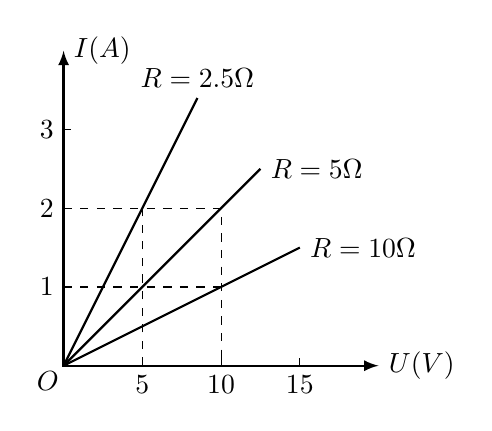
\begin{tikzpicture}[>=latex]
\draw[<->, thick](0,4)node[right]{$I(A)$}--(0,0)--(4,0)node[right]{$U(V)$};
\foreach \x/\xtext in {1/5,2/10,3/15}
{
    \draw(\x,0)node[below]{$\xtext$}--(\x,.1);
    \draw (0,\x)node[left]{$\x$}--(.1,\x);
}
\draw[dashed](0,2)--(2,2)--(2,0);
\draw[dashed](1,0)--(1,2);
\draw[dashed](0,1)--(2,1);
\draw[domain=0:1.7, samples=10, thick] plot(\x, {2*\x})node[above]{$R=2.5\Omega$};
\draw[domain=0:2.5, samples=10, thick] plot(\x, {\x})node[right]{$R=5\Omega$};
\draw[domain=0:3, samples=10, thick] plot(\x, {.5*\x})node[right]{$R=10\Omega$};
\node at (-.2,-.2){$O$};
\end{tikzpicture}
    \caption{}
\end{figure}
从图中可以看出:当导体电阻由5欧增大为10欧时,图
线的斜率变小;当电阻减小为2.5欧时,图线斜率增大。
    \end{solution}
\end{enumerate}




\subsection{练习二}

\begin{enumerate}
    \item 图7.7是滑动变阻器的结构图,涂有绝缘漆的电阻丝密绕在瓷管上,$A$、$B$是它的两个端点,滑动端$P$可在金属杆上移动,它通过金属片与电阻丝接触,把电阻丝和金属杆连接起来.如果把固定端$A$和接线柱$C$接入电路中,当滑动端从$B$向$A$移动时,电路中的电阻就随着变小,说明其道理.
    \begin{figure}[htp]\centering
       \includegraphics[scale=1.5]{fig/7-4.PDF}
        \caption{滑动变阻器}
        \end{figure}

\begin{solution}
    根据电阻定律$R=\rho\ell/S$,
    可知均匀电阻丝的电阻跟它
    的长度成正比。当滑动端$P$从$B$向$A$移动时,接入电路中的
    电阻丝长度变短,所以电阻随着变小。
\end{solution}

    \item 一卷铝导线长100米,横截面积为1${\rm mm}^2$,这卷导线的电阻是多大?

    \begin{solution}
        由电阻定律得$R=\rho\ell/S$,
        查表可知铝的电阻率$\rho=
        2.9\x10^{-8}\Omega\cdot {\rm m}$,则这卷铝线的电阻
\[R=2.9\x 10^{-8}\x\frac{100}{1\x 10^{-6}}=2.9\Omega\]
    \end{solution}
    
    \item 有一段导线,电阻是4欧,把它对折起来作为一条导线用,电阻是多大?如果把它均匀拉长到原来的两倍,电阻又是多大?

    \begin{solution}
已知$R=\rho\ell/S=4$欧,把它对折后$\ell_1=\frac{1}{2}\ell$,
$S_1=2S$,则这时导线电阻
\[R_1=\rho\frac{\frac{1}{2}\ell}{2S}=\frac{1}{4}R=1\Omega\]

把它均匀括长到原来的两倍后,$\ell_2=2\ell$, $S_2=\frac{1}{2}S$,则这时导线电阻
\[R_2=\rho\frac{2\ell}{\frac{1}{2}S}={4}R=16\Omega\]
    \end{solution}
    
    \item 一根做电学实验用的铜导线,长度是60厘米,横截面积是0.5${\rm mm}^2$,它的电阻是多少欧?一根输电用的铜导线,长度是10千米,横截面积是1${\rm cm}^2$,它的电阻是多少欧?为什么做电学实验时可以不考虑连接用的铜导线的电阻,而对输电线路的导线的电阻则需要考虑?

    \begin{solution}
做电学实验用的铜导线的电阻
\[R_1=\rho\frac{\ell_1}{S_1}=1.7\x 10^{-8}\x \frac{0.6}{0.5\x 10^{-6}}=0.02\Omega\]

输电铜导线的电阻
\[R_2=\rho\frac{\ell_2}{S_2}=1.7\x 10^{-8}\x \frac{10\x 10^{3}}{1\x 10^{-4}}=1.7\Omega\]
从计算结果可以看出:做电学实验时,连接用的铜导线的电阻很小,对电路中电流强度的影响甚微,因此可以不予考
虑;而输电线的电阻较大,足以影响电路中的电流强度,所以
需要考虑。
    \end{solution}
    
    \item 一根电阻丝长10米,横截面积是0.2${\rm mm}^2$,两端加上10伏电压时,通过的电流强度是0.2安.这根电阻丝的电阻率是多大?它是用什么材料制作的?

    \begin{solution}
由欧姆定律$I=U/R$,知电阻丝的电阻
\[R=\frac{U}{I}=\frac{10}{0.2}=50\Omega\]
又因$R=\rho\ell/S$,则电阻丝的电阻率
\[\rho=\frac{RS}{\ell}=\frac{50\x0.2\x10^{-6}}{10}=1.0\x 10^{-6}\Omega\cdot {\rm m}\]
查表得知它是用镍铬合金制作的。
    \end{solution}
    
\end{enumerate}



\subsection{练习三}
\begin{enumerate}
    \item 额定电压相同、额定功率不同的两只灯泡,哪个的额定电流大?哪个的电阻大?

    \begin{solution}
    由$P=UI$, 有$I=P/U$。
可见额定电压相同时,灯泡的
额定电流与额定功率成正比,额定功率大的灯泡额定电流大。
因灯泡是纯电阻元件,故$P=U^2/R$, 
即$R=U^2/P$。
可见电阻与额定功率成反比,额定电压相同的两只灯泡,额定功率小的灯泡电阻大。
    \end{solution}
    
    \item 用户保险盒中安装的保险续允许通过的最大电流一般都不大(几个安培),如果在电路中接入功率在1000瓦以上的用电器,如电炉等,就会把保险丝烧断,这是为什么?

    \begin{solution}
因为功率为1000瓦以上的用电器的工作电流为
$I=P/U=\frac{1000}{220}=4.55{\rm A}$以上,把它接入电路后,如果电路中的
电流强度超过保险丝允许通过的最大电流(几安培),就会把
保险丝烧断。
    \end{solution}
    
    \item 日常使用的电功单位是“度”,等于功率为1千瓦的电流在1小时内做的功,又叫千瓦时,1度等于多少焦?

    \begin{solution}
        因$W=Pt$, 故$1\text{度}=1000{\rm W}\x3600{\rm s}=3.6\x10^6{\rm J}$
    \end{solution}
    
    \item 有一个1千瓦、220伏的电炉,正常工作时电流是多少?如果不考虑温度对电阻的影响,把它接在110伏的电压上,它的功率将是多少?

    \begin{solution}
因$P=UI$, 故正常工作时,通过电炉的电流是
\[I=\frac{P}{U}=\frac{1000}{220}=4.55{\rm A}\]
该电炉的电阻为$R=U/I=\frac{220}{4.55}=48.4\Omega$。
把它接到110伏的电压上,它的功率将是
\[P'=\frac{U'}{R}=\frac{110^2}{48.4}=250{\rm W}\]
    \end{solution}
    
    \item 输电线的电阻共计1.0欧,输送的电功率是100千瓦,用400伏的低压送电,输电线上发热损失的功率是多少千瓦?改用1万伏的高压送电呢?

    \begin{solution}
因$P=UI$, 故输电线上电流为$I=P/U$,则输电线上发热损失的功率
\[P_{\text{热}}=I^2R_{\text{线}}=\left(\frac{P}{U}\right)^2R_{\text{线}}\]
当用400伏低压送电时,
\[P_{\text{热}}=\left(\frac{100\x 10^3}{400}\right)^2\x 1.0=6.25\x 10^4{\rm W}=62.5{\rm kW}\]
当用1万伏高压送电时
\[P'_{\text{热}}=\left(\frac{100\x 10^3}{10^4}\right)^2\x 1.0=100{\rm W}=0.1{\rm kW}\]
    \end{solution}
    
    \item 用功率为2千瓦的电炉把2千克的水从20$^\circ$C加热到100$^\circ$C,如果电炉的效率为30\%,需要多少时间?水的比热为$4.2\x10^3{\rm J}/({\rm kg}\cdot {}^\circ {\rm C})$.

    \begin{solution}
把2千克水从$20^{\circ}{\rm C}$加热到$100^{\circ}{\rm C}$需吸收热量
$Q=cm\Delta T$.

设电炉需通电的时间为$t$秒,则电功为
$W=Pt$.

由题设条件电炉的效率$\eta=0.3$, 故
$\eta Pt=cm\Delta T$
所以
\[t=\frac{cm\Delta T}{\eta P}=\frac{4.2\x10^3\x2\x(100-20)}{0.3\x 2000}=1120{\rm s}\]
    \end{solution}
    
\end{enumerate}


\subsection{练习四}
\begin{enumerate}
    \item 电炉和导线是串联的,把它们接入电源后,导线和电炉丝中通过的电流强度是否一样?为什么这时电炉丝热得发红,导线并不热?

    \begin{solution}
因为流过串联电路各电阻的电流强度相等,所以导线
和电炉丝中通过的电流强度是一样的。但由于电流通过导体
产生的热量$Q=I^2Rt$与导体的电阻$R$成正比,电炉丝的电阻
远比导线电阻大且散热又不好,故电炉丝热得发红,而导线并
不热。    
    \end{solution}
    \item 某同学要为游艺晚会准备一棵装有彩色电灯的小松树,如果所用的每只灯泡的额定电压是8伏,用220伏的市电做电源,那么需要将多少只灯泡串联在一起才能接在电源上?

    \begin{solution}
 设需将$n$只灯泡串联起来接在电源上。
因为$U=nU_1$,则
\[n=\frac{U}{U_1}=\frac{220}{8}\approx 28\text{(只)}\]   
    \end{solution}
    \item 一个量程为150伏的电压表,内阻为20千欧,把它与一高电阻串联后接在110伏的电路上,电压表的读数是5伏.求高电阻的阻值是多少?(这是测量高电阻的一种方法)

    \begin{solution}
电压表的读数就是电压表两端的电压。

设电压表内阻为$R_1$, 其两端电压为$V_1$; 高电阻的阻值为
$R_2$, 两端的电压为$U_2$, 串联电路的电流强度为$I$.

因为串联电路两端电压等于各部分电路电压之和,$U=
U_1+U_2$, 所以可求出$R_2$上的电压
\[U_2=U-U_1=110-5=105{\rm V}\]
从$U=IR$, 可得串联电路中的电流强度
\[I=\frac{U_1}{R_1}=\frac{5}{20\x10^3}=2.5\x 10^{-4}{\rm A}\]
于是,高电阻
    \[R_2=\frac{U_2}{I}=\frac{105}{2.5\x 10^{-4}}=4.2\x 10^{5}\Omega=420{\rm k}\Omega\]

    $R_2$也可以利用串联电路的电压分配公式求得.因为
\[\frac{U_1}{R_1}=\frac{U_2}{R_2},\qquad U=U_1+U_2\]
由此可得:
\[R_2=\frac{(U-U_1)R_1}{U_1}=\frac{(110-5)\x 20}{5}{\rm k}\Omega=420{\rm k}\Omega\]
    \end{solution}
    \item 直流电动机线圈的电阻很小,所以起动时的电流很大,这对电动机本身和接在同一电源上的其他用电器都产生不良的后果.为了减小电动机起动时的电流,需要给电动机串联一个起动电阻$R$,如图7.8所示,电动机起动后再将$R$逐渐减小,如果电源电压$U=220$伏,电动机的线圈电阻$r_0=2$欧,那么,
    \begin{enumerate}
        \item 不串联电阻$R$时的起动电流是多大?
        \item 为了使起动电流减小为20安,起动电阻应为多大?
    \end{enumerate}

\begin{figure}[htp]
\centering
\begin{minipage}[t]{0.48\textwidth}
\centering
        \begin{circuitikz}[european,>=stealth]
            \draw(0,0)--(5,0) to  (5,3);
            \draw (0,3) to [vR=$R$] (5,3);
            
            \draw[<->](0,.1) to node [fill=white]{$U$} (0,3-.1);
            \draw (5,1.5) node[elmech]{};
            \draw [fill=white](0,0) circle (2pt);
            \draw [fill=white](0,3) circle (2pt);  
            \node at (5.7, 1.5){$r_0$};
        \end{circuitikz}
    
        \caption{}
        \end{minipage}
\begin{minipage}[t]{0.48\textwidth}
\centering
\begin{circuitikz}[european,>=latex]
    \draw (0,0)--(2,0) to [R=$R_3$] (2,2) to [R=$R_2$] (2,4) to [R=$R_1$] (2,6)--(0,6);
    \draw (2,0)--(4,0)node[right]{$b$};
    \draw [<-](2.2,3)--(4,3)node[right]{$a$};
    \draw [fill=white](4,3) circle (2pt);
    \draw [fill=white](4,0) circle (2pt);      
    \draw [fill=white](0,0) circle (2pt);
    \draw [fill=white](0,6) circle (2pt);   
    \draw[<->](0,.1) to node [fill=white]{$U$} (0,6-.1);
    \node at (2.4,2.7){$P$}; 
        \end{circuitikz}
\caption{}
\end{minipage}
\end{figure}

    \begin{solution}
根据欧姆定律,不串联起动电阻$R$时的起动
电流
\[I=\frac{U}{r_0}=\frac{220}{2}=110{\rm A}\]

串联起动电阻后,电路的总电阻
\[R_{\text{总}}=\frac{U}{I}=\frac{220}{20}=11\Omega\]
因$R_{\text{总}}=R+r_0$, 故起动电阻$R=R_{\text{总}}-r_0=11-2=9\Omega$
    \end{solution}
    \item 图7.9是一个变阻器分压电路,如果电压$U=12$伏,$R_1=350$欧,$R_2=270$欧,$R_3=550$欧,那么,滑动端$P$从$R_2$下端向上移动时,$a$、$b$间的电压将怎样变化?当$P$在$R_2$最下端和最上端时,$a$、$b$间的电压各是多少?

    \begin{solution}
   滑动端$P$从$R_2$下端向上移动,$a$、$b$间的电压将
增大。

当$P$在$R_2$最下端时,$a$、$b$间电压即为$R_3$两端电压。因为
串联电路的电流强度 
\[I=\frac{U}{R_1+R_2+R_3}\]
故\[U_{ab}=IR_3=\frac{UR_3}{R_1+R_2+R_3}=\frac{12\x 550}{350+270+550}=5.6{\rm V}\]

当$P$在$R_2$最上端时,$a$、$b$间电压即为$R_2+R_3$两端的
电压,则
\[U'_{ab}=I(R_2+R_3)=\frac{U(R_2+R_3)}{R_1+R_2+R_3}=\frac{12\x (270+550)}{350+270+550}=8.4{\rm V}\]
    \end{solution}	
\end{enumerate}





\subsection{练习五}
\begin{enumerate}
    \item 电路中需要一个阻值为15千欧的电阻,现在手边只有几只10千欧的电阻,怎样才能组成一个15千欧的电阻?
    

    \begin{solution}
        两只10千欧的电阻并联,其等效电阻
        \[R_{\text{并}}=\frac{1}{2}R=\frac{1}{2}\x 10=5{\rm k}\Omega\]
        再把它跟一只10千欧的电阻串联,总电阻
        \[R_{\text{总}}=R+R_{\text{并}}=10+5=15{\rm k}\Omega\]
        符合题目的要求。   
    \end{solution}
    
    \item 在图7.10所示的电路中,$R_1=10$欧,$R_2=30$欧,$U=6$伏,电键$K$合上前后,
    \begin{enumerate}
        \item 电路中的总电阻各是多少?
        \item 通过$R_1$、$R_2$的电流强度各是多少?
        \item $R_1$、$R_2$上消耗的功率各是多少?
    \end{enumerate}
    \begin{figure}[htp]\centering
        \begin{circuitikz}[european, >=latex]
            \draw (0,0) -- (5,0) to [R=$R_2$] (5,2.5) to [cute open switch] (5,4)-- (0,4);
            \draw (3,0) to [R=$R_1$, *-*] (3,4);
            \draw [fill=white](0,4) circle (2pt);
            \draw [fill=white](0,0) circle (2pt);
    \draw[<->](0,.1)--node [fill=white]{$U$} (0,4-.1);
            \node at (5.3, 3.5){$K$};
        \end{circuitikz}
    
        \caption{}
    \end{figure}	

    \begin{solution}
\begin{enumerate}
    \item 电键$K$闭合前,电路中只有电阻$R_1$, 故总电阻
\[R=R_1=10\Omega\]
电键$K$闭合后,$R_1$与$R_2$并联,总电阻
\[R'=\frac{R_1R_2}{R_1+R_2}=\frac{10\x 30}{10+30}=7.5\Omega\]
\item 电键$K$闭合前,通过$R_1$的电流
\[I_1=\frac{U_1}{R_1}=\frac{6}{10}=0.6{\rm A}\]
通过$R_2$的电流$I_2=0$

电键$K$闭合后,通过$R_1$的电流
\[I'_1=\frac{U}{R_1}=\frac{6}{10}=0.6{\rm A}\]
通过$R_2$的电流
\[I'_2=\frac{U}{R_2}=\frac{6}{30}=0.2{\rm A}\]
\item 电键$K$闭合前,$R_1$上消耗的功率
\[P_1=I_1^2R_1=0.6^2\x10=3.6{\rm W}\]
$R_2$上消耗的功率$P_2=0$.

电键$K$闭合后,$R_1$上消耗的功率
\[P_1'={I_1'}^2R_1=0.6^2x10=3.6{\rm W}\]
$R_2$上消耗的功率 
\[P_2'={I_1'}^2R_2=0.2^2\x30=1.2{\rm W}\]
\end{enumerate}
    \end{solution}
	


    \item 在图7.11所示的电路中,要使通过$R_1$的电流强度不超过5毫安,分流电阻$R_2$应为多大?

    \begin{solution}
因为$R_2$与$R_1$并联,所以
\[U_2=U_1=I_1R_1=5\x10^{-3}\x100=0.5{\rm V}\]
又因通过$R_2$的电流强度$I_2=I-I_1=3-5\x10^{-3}=3{\rm A}$
故分流电阻
\[R_2=\frac{U_2}{I_2}=\frac{0.5}{3}=0.167\Omega\]
    \end{solution}

    \begin{figure}[htp]
        \centering
        \begin{minipage}[t]{0.48\textwidth}
        \centering
                \begin{circuitikz}[european, >=latex, scale=.8]
            \draw (0,0) -- (5,0) to [R=$R_1$] (5,4)--(0,4);
            \draw (3,0) to [R=$R_2$, *-*] (3,4);
            \draw [->] (.5,4)--(1.5,4)node [above]{3A};
            \node at (6.2, 2.4) {5mA};
            \node at (6.2, 1.6) {100$\Omega$};
            \draw [fill=white](0,4) circle (2pt);
            \draw [fill=white](0,0) circle (2pt);
                \end{circuitikz}
            
                \caption{}
                \end{minipage}
        \begin{minipage}[t]{0.48\textwidth}
        \centering
            \begin{circuitikz}[european, >=latex, scale=.8]
                \draw (0,0) -- (5,0) to [R=$R_2$] (5,4) to  [R=$R_1$]  (0,4);
        \draw (5, 1)--(6,1)--(6,3)--(5,3);
        \draw[<->](0,.1)--node [fill=white]{$U$} (0,4-.1);
                \node at (6.3, 2){$L$};
                \draw [fill=white](0,4) circle (2pt);
                \draw [fill=white](0,0) circle (2pt);
                \draw [fill=black](5,1) circle (2pt);
                \draw [fill=black](5,3) circle (2pt);
            \end{circuitikz}
            \caption{}
        \end{minipage}
            \end{figure}

    \item 在图7.12所示的电路中,$L$是跟$R_2$并联的一条导线,下列说法哪些是正确的?

    
    \begin{enumerate}
        \item 通过$R_1$、$R_2$的电流强度$I$相等:
        \[I=\frac{U}{R_1+R_2} \]
        \item $R_1$上的电压$U_1=R_1I_1$,$R_2$上的电压$U_2=R_2I$,导线$L$中的电流为零.
        \item $R_1$上的电压$U_1=U$,$R_2$上的电压为零.
        \item $R_1$中的电流强度$I_1=U/R_1$,导线$L$中的电流强度等于$I_1$;$R_2$中的电流强度为零.
\item $R_2$去掉后,电路中的电阻和电流强度不发生变化.
    \end{enumerate}

    \begin{solution}
(c)、(d)、(e)是正确的。

提示:导线$L$的电阻可忽略不计,即认为$R_L=0$.
    \end{solution}
\end{enumerate}



\subsection{练习六}

\begin{enumerate}
    \item 有一个电流表,内阻为100欧,满度电流为3毫安,要把它改装成量程为3安的安培表,需并联多大的分流电阻?要把它改装为6伏的伏特表,需串联多大的电阻?

    \begin{solution}
在测量了安培的电流时,分流电阻$R$上通过的电流
应该是
\[I_R=I-I_g=3-3\x10^{-3}=2.997{\rm A}\]
由于并联电路中电流强度跟电阻成反比
\[I_gR_g=I_RR\]
所以,需并联的分流电阻值
\[R=\frac{I_g}{I_R}R_g=\frac{3\x10^{-3}}{2.997}\x100=0.1\Omega\]

在测量6伏的电压时,分压电阻两端的电压应该是
\[U_R=U-I_gR_g=6-3\x10^{-3}\x100=5.7{\rm V}\]
所以,需串联的分压电阻值
\[R=\frac{U_R}{I_g}=\frac{5.7}{3\x10^{-3}}=1.9\x10^3\Omega\]
    \end{solution}
    
    \item 电流表的内阻为$R_g$,满度电流为$I_g$.试证明:
     \begin{enumerate}
         \item 要把它改装成量程为$U=nI_gR_g$的伏特表,串联电阻的阻值应为$R_{\text{串}}=(n-1)R_g$;
         \item 要把它改装成量程为$I=nI_g$的安培表,并联电阻的阻值应为$R_{\text{并}}=R_g/(n-1)$.
     \end{enumerate}

     \begin{proof}
\begin{enumerate}
    \item 电流表改装为伏特表时,表头能承受的最大电压
    为$U_g=I_gR_g$.

    由于改装伏特表的量程为$U=nI_gR_g$, 故分压电阻应承受
    的电压$U_R=U-U_g=(n-1)I_gR_g$.

    根据串联电路的电压分配关系
    \[\frac{U_g}{R_g}=\frac{U_R}{R_{\text{串}}}\]
    得串联电阻的阻值
\[R_{\text{串}}=\frac{U_R R_g}{U_g}=\frac{(n-1)I_gR_g}{I_gR_g}R_g=(n-1)R_g\]

    \item 电流表改装为安培表时,表头能承受的最大电流
    为$I_g$.

    由于改装安培表的量程为$I=nI_g$, 故分流电阻应分担的
    电流 $$I_{\text{并}}=I-I_g=(n-1)I_g$$.

    根据并联电路的电流分配关系 $I_gR_g=I_R R_{\text{并}}$, 得并联电阻的阻值
\[R_{\text{并}}=\frac{I_g}{I_R}R_g=\frac{I_g}{(n-1)I_g}R_g=\frac{1}{n-1}R_g\]
\end{enumerate}
     \end{proof}
     
     \item 在第1题中,改装后的安培表的量程比电流表原来的电流量程扩大的倍数$n$是多少?改装后的伏特表比电流表原来的电压量程扩大的倍数$n$又是多少?利用第2题中推出的两个公式,重新计算第1题中的并联电阻和串联电阻,比较两次计算的结果是否相同.

     \begin{solution}
        改装安培表的量程比电流表原来的电流量程扩大的倍数
\[n=\frac{I}{I_g}=\frac{3}{3\x 10^{-3}}=1000\]

改装伏特表的量程比电流表原来的量程扩大的倍数
\[n=\frac{U}{U_g}=\frac{U}{I_gR_g}=\frac{6}{3\x 10^{-3}\x 100}=20\]
由$R_{\text{并}}=\frac{1}{n-1}R_g$,得:
\[R_{\text{并}}=\frac{1}{1000-1}\x 100=0.1\Omega\]
由$R_{\text{串}}=(n-1)R_g$,得:
\[R_{\text{串}}=(20-1)\x 100=1900\Omega=1.9{\rm k}\Omega\]
计算结果均与第1题的计算结果相同。
     \end{solution}
     
     \item 有一安培表,内阻为0.03欧,量程为3安,测量电阻$R$中的电流强度时,本应与$R$串联,如果不注意,错把安培表与$R$并联了(图7.13),将会产生什么后果?假设$R$两端的电压为3伏.
     
\begin{figure}[htp]\centering
    \begin{circuitikz}[european]
\draw (0,0)node[left]{$-$}--(4,0) to [R=$R$] (4,3)--(0,3) node[left]{$+$};
\draw (2.5,0) to [rmeter, t=A, *-*] (2.5, 3);
\draw [fill=white](0,0) circle (2pt);
\draw [fill=white](0,3) circle (2pt);
    \end{circuitikz}

    \caption{}
\end{figure}	

     \begin{solution}
因安培表与$R$并联,故
安培表两端电压跟$R$两端电压
相等,即 $U_A=U_R=3{\rm V}$

这时通过安培表的电流强度
\[I_A=\frac{U_A}{R_g}=\frac{3}{0.03}=100{\rm A}\]
远大于安培表的满度电流3安,安培表将烧毁。
     \end{solution}
     
\end{enumerate}



\subsection{练习七}
\begin{enumerate}
    \item 图7.21是某电路中的一部分,$R_2$、$R_3$、$R_4$是三个电子管的灯丝电阻,阻值分别为$R_2=R_3=84$欧,$R_4=21$欧,分压电阻$R_1=31$欧,$AB$间的电压是28伏,求通过各电子管灯丝的电流强度.
    \begin{figure}[htp]\centering
        \begin{circuitikz}[european, thick]
    \draw (-2,0) node[above]{$A$} to [R=$R_1$] (2,0) to [bulb=$R_2$] (4,0) to [bulb=$R_4$] (7,0) -- (8,0) node[above]{$B$};
    
    \draw (1.5,0)--(1.5,-2) to [bulb=$R_3$] (4.5,-2)--(4.5,0);
    \draw [fill=white](-2,0) circle (2pt);
    \draw [fill=white](8,0) circle (2pt);
    \draw [fill=black](1.5,0) circle (2pt);
    \draw [fill=black](4.5,0) circle (2pt);
    \node at (-2-.3,0){$+$};
    \node at (8+.3,0){$-$};
        \end{circuitikz}
        \caption{}
    \end{figure}	


    \begin{solution}
电路的总电阻
\[R=R_1+R_4+\frac{R_2}{2}=31+21+\frac{84}{2}=94\Omega\]
通过$R_4$的电流强度即电路的总电流强度
\[I=\frac{U_{AB}}{R}=\frac{28}{94}=0.30{\rm A}\]
通过$R_2$和$R_3$的电流强度相等。
\[I_2=I_3=\frac{1}{2}I=\frac{1}{2}\x 0.30=0.15{\rm A}\]
    \end{solution}
    
    \item 图7.22中,电源电压为220伏,各段输电导线上的电阻$r$都为2欧,用电器$R_1$的电阻为200欧,$R_2$的电阻为196欧,$R_1$、$R_2$两端的电压各是多少?
    \begin{figure}[htp]\centering
        \begin{circuitikz}[european, >=latex]
    \draw (0,0)--node [below]{$r$} (3,0)--node[below]{$r$}(5,0) to [R=$R_2$] (5,3)
    --node[above]{$r$}(3,3) --node[above]{$r$}(0,3);
            \draw (3,0) to [R=$R_1$, *-*] (3,3);
    
    
    \draw [<->](0,0.1)--node [fill=white]{220V} (0,3-.1);
    \draw [fill=white](0,0) circle (2pt);
    \draw [fill=white](0,3) circle (2pt);
    
        \end{circuitikz}
    
        \caption{}
    \end{figure}


    \begin{solution}
从图看出$R_2$与两个$r$串联后与$R_1$并联,再与两个$r$
串联,最后接到220伏电源上,并联部分的电阻
\[R_{\text{并}}=\frac{R_1(2r+R_2)}{R_1+2r+R_2}=\frac{200\x (2\x 2+196)}{200+2\x 2+196}=100\Omega\]
电路的总电阻
\[R=2r+R_{\text{并}}=2\x2+100=104\Omega\]
电路的总电流强度
\[I=\frac{U}{R}=\frac{220}{104}=2.12{\rm A}\]
则用电器$R_1$两端的电压
\[U_1=U_{\text{并}}=IR_{\text{并}}=2.12\x 100=212{\rm V}\]

因通过$R_2$的电流强度
\[I_2=\frac{U_{\text{并}}}{2r+R_2}=\frac{212}{2\x 2+196}=1.06{\rm A}\]
故用电器$R_2$两端的电压
\[U_2=I_2R_2=1.06\x196=208{\rm V}\]
    \end{solution}
    
    \item 一个600欧的电阻和一个400欧的电阻串联后接在电压为90伏的电源上,用伏特表测得600欧电阻上的电压为45伏.
    \begin{enumerate}
        \item 伏特表接入电路后,600欧电阻上的电压改变了多少?
        \item 这个伏特表的内阻是多少?
    \end{enumerate}
    
\begin{solution}
\begin{enumerate}
    \item 在未接入伏特表时,电路的电流强度
\[I=\frac{U}{R_1+R_2}=\frac{90}{600+400}=0.090{\rm A}\]
    这时600欧电阻上的电压
 \[   U_1=IR_1=0.090\x600= 54{\rm V}\]
 因伏特表接入电路后,$R_1$两端电压变为45伏,故600欧
 电阻上的电压改变为$54-45=9{\rm V}$。
\item  伏特表接入电路后,600欧电阻上的电压之所以改变,
 是因为伏特表有内阻$R_V$, 它与$R_1$并联,
 因$U_{\text{并}}=45$伏,$U_2=U-U_{\text{并}}=90-45=45{\rm V}=U_{\text{并}}$,故
 \[R_1=R_2=400\Omega\]
由于
\[\frac{1}{R_{\text{并}}}=\frac{1}{R_V}+\frac{1}{R_1}\]
 则伏特表内阻
 \[R_V=\frac{R_{\text{并}}R_1}{R_1-R_{\text{并}}}=\frac{600\x 400}{600-400}=1.20\x 10^3\Omega\]
\end{enumerate}
\end{solution}

    \item 在图7.16中滑动变阻器作分压器使用,负载电阻$R$一端接在变阻器的固定端$A$上,另一端接在滑动端$P$上,滑动端$P$在$AB$间移动时,$R$上就能得到不同的电压.
    \begin{figure}[htp]\centering
        \begin{circuitikz}[european,>=latex]
    
     \draw (0,0) to [R] (5,0) to [cute open switch] (6,0)--(7,0) ;      
     \draw (0,0)--(0,-2);
     \draw (7,0)--(7,-2);
    
     \draw [fill=white](0,-2) circle (2pt);
     \draw [fill=white](7,-2) circle (2pt);
     \draw [fill=black](0,0) circle (2pt);
    
    \draw (0,0) -- (0,1) to [R=$R$] (2.5,1); 
    \draw [->](2.5,1)--node [right]{$P$} (2.5,.2);
    \node at (2-.1,-.4){$A$};
    \node at (3+.1,-.4){$B$};
    \node at (5.5,-.4){$K$};
    
    
    
    \draw [<->](0+.1,-2)--node [fill=white]{$U$} (7-.1,-2);
    
    
       \end{circuitikz}
    
        \caption{}
    \end{figure}

    \begin{enumerate}
        \item 当滑动端从$A$向$B$移动时,$R$上的电压怎样变化?
        \item 如果电压$U=6$伏,变阻器的电阻$R_{AB}=50$欧,负载电阻$R=100$欧,当滑动端$P$在$A$点、$R$点时,$R$上的电压各是多少?
        \item 当$P$在$AB$中点时,$R$上的电压是否为3伏?通过变阻器各部分的电流是否相等?
    \end{enumerate}
    

\begin{solution}
    从图看出,$R$与$R_{AP}$并联后与$R_{PB}$串联。
\begin{enumerate}
    \item 由于
    \[R_{\text{并}}=\frac{R\cdot R_{AP}}{R+R_{AP}}=\frac{R}{1+R/R_{AP}}\]
    当$P$从$A$向$B$移动
时$R_{AP}$由小变大,所以$R_{\text{并}}$也由小变大。又因$R_{\text{并}}$跟$R_{PB}$串
联,根据串联电路中各电阻两端的电压跟它的阻值成正比,可
知$U_{\text{并}}$(即$R$上的电压)将随$R_{\text{并}}$的变大而变大。
\item 当滑动端$P$在$A$点时,$R$被导线短路,故$R$上的电压
为零。

当$P$在$B$点时,$R$与$R_{AB}$并联起来接到$U=6$伏的电源
电压上,故$R$上电压为6伏.
\item 当$P$在$AB$中点时,电器的总电阻
\[R_{\text{总}}=\frac{RR_{AP}}{R+R_{AP}}+R_{PB}=\frac{100\x \frac{1}{2}\x 50}{100+\frac{1}{2}\x 50}+\frac{1}{2}\x 50=45\Omega\]
$R$上的电压
\[U_{\text{并}}=U-U_{PB}=U-\frac{U}{R_{\text{总}}}R_{PB} =6-\frac{6}{45}\x \frac{50}{2}=2.7{\rm V}\]
\end{enumerate}

因通过变阻器$PB$段的电流等于电路的总电流强度,而
通过变阻器$AP$段的电流只是总电流的一部分,总电流的另
一部分经$R$分流。所以$P$在$AB$中点时,通过变阻器各部分
的电流不相等。
\end{solution}

\end{enumerate}



\subsection{练习八}
\begin{enumerate}
    \item 电源的电动势为1.5伏,内电阻为0.12欧,外电路的电阻为1.28欧,求电路宁的电流强度.

    \begin{solution}
根据闭合电路欧姆定律$I=\dfrac{\mathcal{E}}{R+r}$,
可求电路中电流
强度
\[I=\dfrac{\mathcal{E}}{R+r}=\frac{1.5}{1.28+0.12}=1.07{\rm A}\]
    \end{solution}
    
    \item 把一个定值电阻和电源连成图7.17所示的电路,可以测得电源的内电阻,定值电阻$R$为10欧,合上开关$K$时,伏特表的读数为5.46伏,打开$K$时,伏特表的读数为6.0伏.求电源的内电阻为多少.
\begin{figure}[htp]
    \centering
    \begin{circuitikz}[european]
        \draw(0,0)--(5,0) to [R=$R$](5,3) to  [cute open switch] (2,3)--(0,3) to[battery2] (0,0);
        \draw (2,0) to [rmeter, t=V, *-*] (2,3);    
        \node at (7/2,3)[above] {$K$}    ;
            \end{circuitikz}    
    \caption{}
\end{figure}

    \begin{solution}
因断开$K$时,伏特表
的读数为电源电动势,故电源
电动势$\mathcal{E}=6.0$伏.

合上开关$K$时,伏特表的
读数为定值电阻$R$两端的电压。由闭合电路欧姆定律$I=\dfrac{\mathcal{E}}{R+r}$
和部分电路欧姆定律$U=IR$,有
\[U=\frac{\mathcal{E}}{R+r}R\]
则电源内电阻
\[r=\frac{\mathcal{E}R}{U}-R=\frac{6.0\x 10}{5.46}-10=1\Omega\]
    \end{solution}
    
    \item 在图7.18所示的电路中$\mathcal{E}=9.0$伏,$r=3.0$欧,$R=15$欧,当$K$闭合时,$U_{AB}$是多少?当$K$打开时,$U_{AB}$又为多少?

    \begin{solution}
        当$K$闭合时,电路的电流强度为
\[I=\dfrac{\mathcal{E}}{R+r}=\frac{9.0}{15+3.0}=0.50{\rm A}\]
则\[U_{AB}=IR=0.50\x 15=7.5{\rm V}\]
当$K$断开时,$U_{AB}=\mathcal{E}=9.0{\rm V}$
    \end{solution}

    \begin{figure}[htp]\centering
        \begin{minipage}[t]{0.48\textwidth}
    \centering
    \begin{circuitikz}[european, xscale=.8]
        \draw(0,0) to [battery2] (6,0) node [below]{$B$} to[cute open switch] (6,2) to[R=$R$] (0,2)node [above]{$A$}--(0,0) ;
        
        \node at (6,1)[right]{$K$};
        
        \node at (3,-.5)[below]{$\mathcal{E}\;  r$};
            \end{circuitikz}
        
            \caption{}
        \end{minipage}
    \begin{minipage}[t]{0.48\textwidth}
    \centering
            \begin{circuitikz}[european,>=latex, yscale=.8]
        \draw (0,0)to [battery2] (6,0)--(6,2)to [rmeter, t=V, *-*] (0,2) to [rmeter, t=A] (0,0);
        \draw (0,2)--(0,4)--(2,4) to [R] (4,4)--(4.5,4)to [cute open switch] (6,4)--(6,2);
                \draw (1.5,4) to (1.5,4.7)--(3,4.7);
                \draw [->](3,4.7)--(3,4.2);
            \end{circuitikz}
        
            \caption{}\end{minipage}
        \end{figure}    
    
    \item 利用图7.19所示的电路可以测出电源的电动势和内电阻.当变阻器的滑动端在某一位置时,安培表和伏特表的读数分别是0.20安和1.98伏,改变滑动端的位置后,两表的读数分别是0.40安和1.96伏,求电池的电动势和内电阻.

    \begin{solution}
        根据闭合电路的欧姆定律,可列出方程组
\[\begin{split}
    \mathcal{E}&=I_1R_1+I_1 r=U_1+I_1r\\
    \mathcal{E}&=I_2R_2+I_2 r=U_2+I_2r\\
\end{split}\]
消去$\mathcal{E}$,可得
\[U_1+I_1r=U_2+I_2r\]
所以,电源的内电阻
\[r=\frac{U_1-U_2}{I_2-I_1}=\frac{1.98-1.96}{0.40-0.20}=0.1\Omega\]
把$r$的值代入$\mathcal{E}=U_1+I_1r$中,可求得电源电动势
\[\mathcal{E}=1.98+0.20\x 0.1=2.00{\rm V}\]
    \end{solution}
    
\end{enumerate}


\subsection{练习九}

\begin{enumerate}
    \item 试分析说明:外电路中的电阻发生变化时为什么会影响路端电压的变化.

    \begin{solution}
根据闭合电路欧姆定律$I=\dfrac{\mathcal{E}}{R+r}$
可知,就某个电源
来说,由于电动势$\mathcal{E}$和内电阻$r$都是一定的,因此外电路电阻
$R$发生变化时电路的电流强度$I$将发生变化。而路端电压$U=\mathcal{E}-Ir$, 所以当$R$变化导致$I$变化时,$U$必然变化.
    \end{solution}
    
    \item 在两个电路中,电源的电动势相同,但内电阻不同,当它们的外电路中流过的电流相同时,哪个电路的路端电压大?

    \begin{solution}
        由路端电压$U=\mathcal{E}-Ir$可知,若两个电路的$\mathcal{E}$相同、$I$
        相同时,内电阻$r$小的电路路端电压较大。
    \end{solution}
    
    \item 在图7.32所示的电路中,当$P$由左向右滑动时,安培表和伏特表的读数怎样变化?$P$的位置在何处,伏特表的
指示更接近于电源的电动势?

\begin{figure}[htp]\centering
    \begin{circuitikz}[>=latex, european]
\draw (0,0) to [battery2] (6,0)--(6,1) to [rmeter, t=V, *-*] (0,1)--(0,0);
\draw (0,1)--(0,2) to [rmeter, t=A] (2,2) to[R] (6,2)--(6,1);
\draw (6,2)--(6,3)--(4,3);
\draw [->](4,3)--node [left]{$P$}(4,2.2);
\fill [white] (6-.02,2.2) rectangle (4.58,1.8);
    \end{circuitikz}
    \caption{}
\end{figure}


\begin{solution}
    当$P$由左向右滑动时,电路中的电阻$R$变大,由$I=\dfrac{\mathcal{E}}{R+r}$
    可知,安培表的读数即电路中的电流强度将变小;由$U=\mathcal{E}-Ir$可知,伏特表的读数即路端电压将变大。因$R$越大,
    $I$越小,$U$就越大,也就越接近电源电动势;所以当$P$在最右
    端时,$R$值最大,伏特表的示数更接近于电源电动势。
\end{solution}

\item 发电机的电动势为240伏,内电阻为0.40欧,给200盏电阻均为1210欧的电灯供电,电灯上的电压是多大?如果
再接入100盏同样的电灯,电灯上的电压又是多大?利用所得的结果说明:电路中的用电器增多时,加在用电器上的电压将
怎样变化?

\begin{solution}
给200盏相同电灯供电时,外电路总电阻
\[R=\frac{1210}{200}=6.05\Omega\]
这时电路中总电流强度
\[I=\dfrac{\mathcal{E}}{R+r}=\frac{240}{6.05+0.40}=37.2{\rm A}\]
则电灯上的电压
\[U=\mathcal{E}-Ir=240-37.2\x0.40=225{\rm V}\]
如再接入100盏同样的电灯,外电路总电阻
\[R'=\frac{1210}{300}=4.03\Omega\]
同理可求这时电灯上的电压
\[U'=\mathcal{E}-I'r=\mathcal{E}-\frac{\mathcal{E}}{R'+r}r=240-
\frac{240}{4.03+0.40}\x 0.40=218{\rm V}\]
从计算结果可以看出:电路中用电器增多时,加在用电器
上的电压将减小。
\end{solution}

\end{enumerate}




\subsection{练习十}
\begin{enumerate}
    \item 每个铅蓄电池的电动势为2.0伏,想用它们给一个额定电压为6伏的用电器供电,应该怎么办?

    \begin{solution}
由于用电器的额定电压高于单个电池的电动势,可采用串联电池组供电。

依题意蓄电池内阻不计,有$U=\mathcal{E}_{\text{串}}=n\mathcal{E}$,
故
\[n=\frac{U}{\mathcal{E}}=\frac{6}{2.0}=3\]
应当用3个2.0伏的蓄电池串联起来供电。
    \end{solution}
    
    \item 每节干电池的电动势为1.5伏,允许通过的最大电流为0.05安.现在需要一个电动势为6伏,最大电流为0.1安的电源,应该怎么办?

    \begin{solution}
因所需总电动势大于单个电池电动势,应采用串联
电池组.需由$p$个电池串联而成,$\mathcal{E}_{\text{串}}=p\mathcal{E}$.
则
\[p=\frac{\mathcal{E}_{\text{串}}}{\mathcal{E}}=\frac{6}{1.5}=4\]
又因所需电流大于单个电池允许通过的最大电流,应把
几个跟上述串联电池组相同的电池组并联起来组成混联电池
组。设需由$q$个串联电池组并联而成,$I_{\text{总}}=qI$.
则
\[q=\frac{I_{\text{总}}}{I}=\frac{0.1}{0.05}=2\]
所需电池总数 $m=pq=4\x2=8$

要实现题目提出的要求,可用8节干电池,每4节串联成
一组,再将两组并联起来供电。
    \end{solution}
    
    \item 有10个相同的蓄电池,每个蓄电池的电动势为2.0伏,内电阻为0.04欧,把这些蓄电池接成串联电池组,外接它阻为3.6欧.求电路中的电流强度和电池组两端的电压.

    \begin{solution}
因$\mathcal{E}_{\text{串}}=n\mathcal{E}$, $r_{\text{串}}=nr$, 由闭合电路欧姆定律得
\[I=\frac{\mathcal{E}_{\text{串}}}{R+r_{\text{串}}}=\frac{n\mathcal{E}}{R+nr}=\frac{10\x 2.0}{3.6+10\x 0.04}=5.0{\rm A}\]
电池组两端电压
\[U=\mathcal{E}_{\text{串}}-Ir_{\text{串}}=n\mathcal{E}-Inr=10\x 2.0-5.0\x 10\x 0.04=18{\rm V}\]
    \end{solution}
    
    \item 找一个半导体收音机,打开看看里面有几节干电池,是怎样连接的,算一算这个收音机的电源电压是多少.

    \begin{solution}
        一般半导体收音机的电源是由4节1.5伏的干电池
        串联而成.电源电压为$n\mathcal{E}=4\x1.5=6{\rm V}$

        注意:此题答案不是唯一的,例如有不少半导体收音机的电源是由3节干电池串联而成。
    \end{solution}
    
    \item 把两节干电池串联起来组成电池组,用伏特表量出电池组的电动势.再把三个小灯泡照图7.21依次连入电路中,注意每增加一个小灯泡时伏特表读数的变化,说明伏特表的读数为什么会发生变化.这个变化表明了什么?

    \begin{figure}[htp]\centering
        \begin{circuitikz}[european]
    %\draw (0,3)--(6,3) to[lamp] (6,0)--(0,0) to [battery](0,3);
    \draw (0,0)--(6,0) to [lamp] (6,3)--(0,3) to [battery](0,0);
    
    \draw (1.5,0) to [rmeter,t=V, *-*] (1.5,3);
    \draw (4,0) to [lamp, *-*] (4,3);
    \draw (5,0) to [lamp, *-*] (5,3);
    
        \end{circuitikz}
    
        \caption{}
    \end{figure}

    \begin{solution}
        每增加一个灯泡,伏特表的读数就减小一次。因为电
        池组的总电动势和总内阻保持不变,当电源的并联负载不断
        增加时,外电路的总电阻将不断减小,电路的电流强度
$I=\dfrac{\mathcal{E}_{\text{总}}}{R+r_{\text{总}}}$
        将不断增大,导致伏特表的读数(即路端电压)$U=\mathcal{E}_{\text{总}}-Ir_{\text{总}}$不断减小。这个变化表明电路的路端电压随外电阻
        减小而减小。
    \end{solution}
    
\end{enumerate}






\subsection{练习十一}
\begin{enumerate}
    \item 在课本图7.37甲中,如果安培表的读数是0.2安,伏特表的读数是30伏,根据这些数据算出的$R$的阻值是多大?如果已知伏特表的内阻是3千欧,那么,$R$的真实值是多大?采用这种接法时,算出的$R$值比真实值大还是小?

    \begin{solution}
        $R$的计算值
        \[R'=\frac{U}{I}=\frac{30}{0.2}=150\Omega\]
        如考虑伏特表的内阻,则伏特表与$R$并联的等效电阻值
\[R_{\text{并}}=\frac{U}{I}=\frac{30}{0.2}=150\Omega\]
因为$R_{\text{并}}=\dfrac{R_VR}{R_V+R}$,所以,$R$的真实值
\[R=\frac{R_VR_{\text{并}}}{R_V-R_{\text{并}}}=\frac{3000\x 150}{3000-150}=158\Omega\]
可见算出的$R$值比真实值小。
    \end{solution}
    
    \item 在课本图7.37乙中,如果伏特表的读数是5伏,安培表的读数是0.5安,根据这些数据算出的$R$的阻值是多大?如果已知安培表的内阻是0.2欧,那么,$R$的真实值是多大?采用这种接法时,算出的$R$值比真实值大还是小?

    \begin{solution}
$R$的计算值
\[R'=\frac{U}{I}=\frac{5}{0.5}=10\Omega\]
如考虑安培表的内阻,则安培表与R串联的等效电阻值
\[R_{\text{串}}=\frac{U}{I}=\frac{5}{0.5}=10\Omega\]
因为$R_{\text{串}}=R+R_A$, 
所以,$R$的真实值
\[R=R_{\text{串}}-R_A=10-0.2=9.8\Omega\]
可见算出的$R$值比真实值大。
    \end{solution}
    
    \item 已知伏特表的内阻为5千欧,安培表的内阻为0.2欧,如果用它们来测量一个线圈的电阻,估计这个线图的电阻大约为几个欧姆,那么,怎样连接电路测得的结果误差较小?画出电路图.

    \begin{solution}
        从题目已知条件可以看出待测电阻的阻值远小于伏
        特表的内阻,所以采用安培表外接的方式测得结果误差较小。
        如图7.22所示.
\begin{figure}[htp]\centering
    \begin{circuitikz}[european, scale=.8]
\draw (0,0) to [rmeter, t=A] (2,0) to (2.5,0) to [R=$R$, *-*] (5,0)--(6,0);
\draw (2.5,0)--(2.5,1.5) to [rmeter, t=V] (5,1.5)--(5,0);
    \end{circuitikz}
    \caption{}
\end{figure}

    \end{solution}
    
    \item 在课本图7.40中,$R$为15欧,电桥平衡时,$\ell_1$为0.45米,$\ell_2$为0.55米,求待测电阻$R_x$.

    \begin{solution}
        因电桥平测时有
\[\frac{R_x}{R}=\frac{\ell_2}{\ell_1}\]
        所以,待测电阻$R_x$的值
\[R_x=\frac{\ell_2}{\ell_1}R=\frac{0.55}{0.45}\x 15=18\Omega\]
    \end{solution}
    
    \item 在课本图7.40中,如果$AB$支路发生断路,当滑动触头
    $D$从$A$移向$C$时,电流表$G$中的电流如何变化?如果$BC$支路发生断路,当$D$从$A$移向$C$时,电流表$G$中的电流又如何变化?

    \begin{solution}
        可以认为$A$、$C$间电压保持不变。设电阻线$AD$段
        电阻值为$R_1$, $DC$段电阻值为$R_2$.

        当$AB$支路断路时,$R_{DC}=\dfrac{(R_x+R_g)R_2}{R_x+R_gR_2}$
        与$R_1$串联,随滑动
        触头$D$从$A$移向$C$, $R_1$增大,$R_2$减小使$R_{DC}$减小.根据串联
        电路中各电阻两端电压跟它的阻值成正比,$R_{DC}$两端的电压
$U_{DC}$将减小,导致电流表G中电流$I=\dfrac{U_{DC}}{R_x+R_g}$
减小。

当$BC$支路断路时,$R_{AD}=\dfrac{(R+R_g)R_1}{R+R_g+R_1}$
与$R_2$串联,随滑
动触头$D$从$A$移向$C$, $R_2$减小,$R_1$增大使$R_{AD}$增大,根据串
联电路中各电阻两端电压跟它的阻值成正比,$R_{AD}$两端的电
压$U_{AD}$将增大,导致电流表G中电流$I=\dfrac{U_{AD}}{R+R_g}$增大。
    \end{solution}
    
\end{enumerate}






\subsection{习题}

        \begin{figure}[htp]
            \centering
            \begin{minipage}[t]{0.48\textwidth}
            \centering
            \begin{circuitikz}[european, scale=.7, >=stealth]
        
                \draw (0,0) --(4,0) to [R=$R$] (4,5)--(3,5); 
            \draw(1,5)--(0,5)to [battery2] (0,0);
        \draw (2,0) to [C=$C$, *-] (2,4);
        \node at (2,-.5){$b$};
        \draw [ultra thick ] (2,5.25)--(2,4);
        \draw [->] (2,5.25) arc (90:60:1.5);
        \draw [->] (2,5.25) arc (90:120:1.5);
        
        
        \draw (2,4) [fill=white] circle (1.5pt)node[left]{$a$};
        \draw (1,5) [fill=white] circle (1.5pt)node[above]{1};
        \draw (3,5) [fill=white] circle (1.5pt)node[above]{2};\draw (2,5.25) [fill=white] circle (1.5pt);
        
                \end{circuitikz}
            \caption{}
            \end{minipage}
            \begin{minipage}[t]{0.48\textwidth}
            \centering
            \begin{circuitikz}[european, scale=1.5]
    
                \draw (0,0) --(1,0) to [rmeter, t=mA] (2,0); 
                \draw [dashed](2,0)--(3,0)--node[right]{$B$}(3,2)--(2,2);
                \draw (0.8,0) to [rmeter, t=V, *-*] (.8,2); 
            \draw(2,0)--node[right]{$E$}(2,2)--(0,2)to [battery] (0,0);
            \node at (-.5,1){$A$};
                \end{circuitikz}
            \caption{}
            \end{minipage}
            \end{figure}



\begin{enumerate}
    \item 在图7.23中,电键可以向左扳将$a$与1接通,也可以向右扳将$a$与2接通,电键接通1的瞬间,电流的方向怎样?
接通1后再向右扳电键,将$a$与2接通,接通2的瞬间,电流的方向又怎样?

\begin{solution}
    电键$K$接通1的瞬间,电源给电容器$C$充电.充电
    电流的方向从电源正极流出,负极流入.电键接通1后再接
    通2的瞬间,已充电的电容器$C$通过电阻$R$放电。放电电流
    的方向从$C$的上极板流出经$R$流入$C$的下极板。
\end{solution}

\item $A$和$B$两地相距40千米,从$A$到$B$的两条输电线的总电阻为800欧,如果在$A$、$B$之间的某处$E$两条电线发生短路(图7.24),可用伏特表、毫安表和电池组检查出发生短路的地点.如果在$A$处测得伏特表的读数是10伏,毫安表的读数是40毫安,求短路处$E$到$A$的距离.

\begin{solution}
    从$A$到$E$的两条输电线的电阻为
\[R=\frac{U}{I}=\frac{10}{40\x 10^{-3}}=250\Omega\]
因为$\dfrac{AE}{AB}=\dfrac{R}{800\Omega}$,所以,短路处$E$到$A$的距离
\[AE=\frac{R}{800\Omega}AB=\frac{250}{800}\x 40=12.5{\rm km}\]
\end{solution}

\item 有两个灯泡,一个是110伏、100瓦,一个是110伏、
40瓦,把它们串联后接入220伏的电路中使用行不行?为什么?有一个变阻器,把它怎样连入电路中可以使两灯泡正常发光?这时变阻器的阻值应调至多大?

\begin{solution}
110伏、100瓦灯泡的电阻
\[R_1=\frac{U^2}{P_1}=\frac{110^2}{100}=121\Omega\]
110伏、40瓦灯泡的电阻
\[R_2=\frac{U^2}{P_2}=\frac{110^2}{40}=303\Omega\]
由于$R_2>R_1$, 它们串联起来接入220伏电路中使用时,
$U_2$将大于$U_1$, 
\[U_2=\frac{R_2}{R_1+R_2}U=\frac{303}{121+303}\x 220=157{\rm V}\]
可见,40瓦灯泡实际承担的电压已大于自身的额定电压,会
被烧毁,所以这样连接不行。

如要使两灯串联后又都能正常发光,可将变阻器与40瓦
灯泡并联,使它们的等效电阻与100瓦灯泡的电阻相等。这
样,两灯各分担110伏电压,均等于各自的额定电压.设这时
变阻器的阻值为$R$, 则有
\[R_1=R_{\text{并}}=\frac{R_2R}{R_2+R}\]
所以,变阻器的阻值应调到
\[R=\frac{R_1R_2}{R_2-R_1}=\frac{121\x 303}{303-121}=201\Omega\]
\end{solution}

\item 有一用电器$W$,额定电压为100伏,额定功率为150瓦,用120伏的电源供电.为了使用电器能正常工作,用一
电阻为210欧的变阻器进行分压(图7.25).$R_1$、$R_2$为多大时,用电器才能正常工作?

\begin{solution}
先求出用电器$W$的电阻值。
\[R_W=\frac{U^2_W}{P_W}=\frac{100^2}{150}=66.7\Omega\]
因为$R_2$与$R$并联后再与$R_1$串联,根据
串联电路的电压分配关系可得:
\[U_1:U_W = R_1:\frac{R_WR_2}{R_W+R_2}\]
把$R_1=R-R_2$和$U_1=U-U_W$代入上式,整理后得
\[R_2^2+\left(\frac{U}{U_m}R_W-R\right)R_2-RR_W=0\]
将$U=120$伏,$U_m=100$伏,$R_W=66.7$欧,$R=210$欧代入上式
得
\[R_2^2-130\cdot R_2-14000=0\]
解方程(舍去负根)得$R_2=200$欧,$R_1=210-200=10$欧.

\end{solution}

\begin{figure}[htp]
	\centering
	\begin{minipage}[t]{0.48\textwidth}
	\centering
	\begin{circuitikz}[european, scale=1.3, >=stealth]
		\draw [->](0,0)--(2,0)--(3,0)to [R=$W$](3,2)--(2.15,2);
		\draw (2,0)--(2,1) to [R] (2,3)--(0,3);
		
		\draw[<->] (0,.05)--node[fill=white]{$U$}(0,3-.05);
		\draw (2,0) [fill=black] circle (1.2pt);
		\draw (0,0) [fill=white] circle (1.2pt);
		\draw (0,3) [fill=white] circle (1.2pt);
		\node at (1.5,1.5){$R_2$};\node at (1.5,2.5) {$R_1$};
			\end{circuitikz}	\caption{}
	\end{minipage}
	\begin{minipage}[t]{0.48\textwidth}
	\centering
	\begin{circuitikz}[european, scale=1, >=stealth]
		\draw (-2,0) to [R=$R_1$, *-*] (0,0) to  [R=$R_2$, *-*] (2,0);
		\draw (-2,-1.5)--(-2,1.5) to [rmeter, t=G] (2,1.5)--(2,-1.5);
		\draw (0,0)--(0,-1.5);
		\draw (0,-1.5) [fill=white] circle (1.5pt) node[right]{$b$};
		\draw (-2,-1.5) [fill=white] circle (1.5pt)node[right]{$a$};
		\draw (2,-1.5) [fill=white] circle (1.5pt)node[right]{$c$};
		\node at (0,-1.5)[below]{1A}; \node at (0,1.1)[below]{$R_3$};
		\node at (2,-1.5)[below]{0.1A};
		\draw [dashed](2.5,2.2) rectangle (-2.5, -1);
		
			\end{circuitikz}
	\caption{}
	\end{minipage}
	\end{figure}

\item 图7.26所示的是有两个量程的安培表,当使用$a$、$b$两端点时,量程为1安,当使用$a$、$c$两端点时,量程为0.1安.已知电流表的内阻$R_g$为200欧,满度电流$I_g$为2毫安,求电阻$R_1$和$R_2$.


    \begin{solution}
当使用$a$、$b$两端点时,$R_g$与$R_2$串联后与$R_1$并联,
则有
\[I_g(R_g+R_2)=(I-I_g)R_1\]
当使用$a$、$c$两端点时,$R_1$与$R_2$串联后与$R_g$并联,则有
\[I_gR_g=(I'-I_g)(R_1+R_2)\]
代入题设数据得
\[\begin{cases}
    2\x10^{-3}\x(200+R_2)=(1-2\x10^{-3})\x R_1\\
2\x10^{-3}\x200=(0.1-2\x10^{-3})\x(R_1+R_2)
\end{cases}\]
化简后有
\[\begin{cases}
   200+R_2=499R_1\\
200=49\x(R_1+R_2) 
\end{cases}\]

上述二式联立求解可得:$R_1=0.41$欧,$R_2=3.67$欧.
    \end{solution}
    
\item 在课本图7.27中,不用安培表,改用伏特表能不能测出电源的电动势和内电阻?画出伏特表应怎祥接入电路,说明要取得哪些数据,写出计算电动势和内电阻的公式.

\begin{solution}
    不用安培表,改用伏特表能够测出电源电动势和内
    电阻.电路图如图7.27所示.

    将开关先后扳到位置1和位置2, 分别测出$R_1$和$R_2$接
    入电路时的伏特表读数$U_1$和$U_2$. 计算电动势和内电阻的公
    式可根据闭合电路欧姆定律列出方程组
\[\begin{cases}
    \mathcal{E}=U_1+\dfrac{U_1}{R_1}r\\
    \mathcal{E}=U_2+\dfrac{U_2}{R_2}r\\
\end{cases}\]
联立求解得出:
\[\mathcal{E}=\frac{U_1U_2(R_1-R_2)}{U_2R_1-U_1R_2},\qquad r=\frac{(U_1-U_2)R_1R_2}{U_2R_1-U_1R_2}\]
\end{solution}

\begin{figure}[htp]\centering
    \begin{minipage}[t]{0.48\textwidth}
    \centering
\begin{circuitikz}[european]

    \draw (.5,2.5)--(0,2.5)--(0,0) to [battery2] (5,0)--(5,3);
\draw(0,1) to [rmeter, t=V, *-*] (5,1);
\draw(1.5,3) to [R=$R_1$] (5,3);
\draw(1.5,2) to [R=$R_2$] (5,2);

\draw[thick](.5,2.5)node[below]{$K$}--(1.5,2.9);
\draw(1.5,3) [fill=white]circle(1.5pt)node[above]{$1$};
\draw(1.5,2) [fill=white]circle(1.5pt)node[below]{$2$};
\draw(.5,2.5) [fill=white]circle(1.5pt);
\node at (2.2,0)[below]{$\mathcal{E}$};
\node at (2.8,0)[below]{$r$};
    \end{circuitikz}
    \caption{}
    \end{minipage}
    \begin{minipage}[t]{0.48\textwidth}
    \centering
    \begin{circuitikz}[european, xscale=.8]
\draw (0,0)--(8,0) to [lamp] (8,3)--(3,3) to [R=$R$] (0,3) to (0,0);
\draw (3,0)--(3,3);
\draw (5,0)to [lamp] (5,3);
\draw [dashed](6.5,0)to [lamp] (6.5,3);        
\draw (0,1.5) node[elmech]{$F$};
\draw (3,1.5) node[elmech]{$M$};
\node at (1,1.5){$\mathcal{E},\; r$};
\draw [fill=black](3,3) circle (2pt);
\draw [fill=black](5,3) circle (2pt);
\draw [fill=black](6.5,3) circle (2pt);
\draw [fill=black](3,0) circle (2pt);
\draw [fill=black](6.5,0) circle (2pt);
\draw [fill=black](5,0) circle (2pt);
    \end{circuitikz}
    \caption{}
    \end{minipage}
    \end{figure}


\item 在图7.28中,用一台直流发电机$F$给一台电动机$M$和一些电灯供电.已知发电机的电动势$\mathcal{E}=240$伏,内电阻$r=1$欧,输电线的总电阻$R=3$欧,电动机的工作电流为3安,供给电灯的总电流为9安,求电灯和电动机两端的电压.

\begin{solution}
电路的总电流强度
\[I=I_M+I_{\text{灯}}=3+9=12{\rm A}\]
路端电压
\[U=\mathcal{E}-Ir=240-12\x1=228{\rm V}\]
则电灯和电动机两端的电压
\[U'=U-U_R=U-IR=228-12\x3=192{\rm V}\]
\end{solution}


\item 现有电动势为1.5伏,内电阻为1欧的电池若干,每个电池允许输出的电流为0.05安,又有不同阻值的电阻可作为分压电阻,试设计一种电路,使额定电压为6伏、额定电流为0.1安的用电器正常工作,画出电路图,并标明分压电阻的值.

\begin{solution}
    按题意要使用电器正常工作,应采用混联电池组,设
    它由$p$个电池串联为一组,$q$组并联而成。

    要使用电器两端的电压等于额定电压6伏,必须让每组
    串联电池输出的电压$U$满足以下关系:
\[U=p\mathcal{E}-0.05\x pr\ge 6\]
即:\[p\x 1.5-0.05\x r\ge 6\]
则$p$至少要取5。

要使用电器通过的电流等
于额定电流,又不致损坏电池,应满足$0.1=q\x0.05$,则$q=2$。

因此,需将5只电池串联成一组,再将两组并联使用.这
种混联电池组的电动势$\mathcal{E}_{\text{总}}=7.5$伏,内阻
\[r_{\text{总}}=\frac{5\x 1}{2}=2.5\Omega\]

因电池组的输出电压
\[U=5\x1.5-0.05\x5\x1=7.25{\rm V}\]
大于用电器的额定电压,故应给用电器串联一个分压电阻$R$. 

由于$\mathcal{E}_{\text{总}}=Ir_{\text{总}}+IR+U_{\text{额}}$,
式中的$U_{\text{额}}=6$伏,是用电器的额定电压,所以分压电阻
\[R=\frac{\mathcal{E}_{\text{总}}-Ir_{\text{总}}-U_{\text{额}}}{I}=\frac{7.5-0.1\x 2.5-6}{0.1}=12.5\Omega\]
整个电路如图7.29所示.

\begin{figure}[htp]
    \centering
\begin{circuitikz}[european,scale=.8]
\draw (0,4)--(0,0) to [R](3,0) to [R](5,0)--(5,4);
\draw(0,4) to [battery] (5,4);
\draw(0,2) to [battery, *-*] (5,2);
\node at (1.5,-.3)[below]{$R=12.5\Omega$};
\node at (4,-.3)[below]{用电器};

\end{circuitikz}
    \caption{}
\end{figure}

\end{solution}

\item 用伏安法测电阻,如果所用的安培表的内阻$R_A=0.1$
欧,伏特表的内阻$R_V=1000$欧,那么,用课本图7.37所示的两种不同接法测量$R=1$欧的电阻时,哪种方法产生的误差较小?测量$R=500$欧的电阻时,哪种方法产生的误差较小?测量较小的电阻和较大的电阻,各应采用什么方法?

\begin{solution}
    由题设条件可看出:测量$R=1$欧的电阻时,$R\ll R_V$,
    采用课本图7.37甲的接法产生的误差较小;测量$R=500$欧
    的电阻时,$R\gg R_V$, 采用课本图7.37乙的接法产生的误差较
    小.测量较小的电阻应采用课本图7.37甲所示的安培表外
    接法,测量较大电阻应采用课本图7.37乙所示的安培表内
    接法。
\end{solution}

\item 在课本图7.40中,滑动触头$D$从$A$向$C$移动时,电流
表中都有电流通过,但电流强度逐渐减小,这时可能是什么地方发生了断路?如果电流表指示的电流强度逐渐增大,又可能是什么地方发生了断路?

\begin{solution}
    电流表示数逐渐减小,可能$AB$支路发生断路;电流
    表示数逐渐增大,可能$BC$支路发生断路。(具体分析过程可
    参考练习十一第5题的解答)
\end{solution}

\item 在课本图7.40中,无论在从$A$经电源到$C$的电路中发
生断路,还是从$B$经电流表到$D$的电路中发生断路,在按下滑动触头时都没有电流通过电流表.用什么办法可以把这两种情况区别开来?

\begin{solution}
    可将滑动触头$D$处接线断开,然后把$D$处与电流表相
    连的接线线端跟电源正、负极瞬时接触。如果电流表都不偏
    转,说明$B$经电流表到$D$的电路发生了断路;如接触电源正极时,电流表偏转,说明从$A$到电源正极的电路发生了断路;如
    接触电源负极时电流表偏转,说明从电源负极到$C$的电路发
    生了断路。
\end{solution}

\end{enumerate}



\section{参考资料}
\subsection{超导电现象}
1911年荷兰科学家昂尼斯发现,水银的电阻率并不象预
料的那样随温度降低逐渐减小,而是在绝对温度4.15K附近
突然减小到测不出来。现在用最精确的方法估计,其电阻率
小于$10^{-25}$欧·米,而良导体之一的铜,即使是最纯的铜,在温
度为4.15K时的电阻率也有$10^{-11}$欧·米,因此,完全可以认为
在4.15K附近水银的电阻已趋消失.某些金属、合金和化合
物,在温度降到绝对零度附近某一特定温度时,它们的电阻率
会突然减小到无法测量的现象叫超导现象,处于这种状态的
导体叫超导体,每一种超导物质都在特定的温度下转变为超
导体。这个温度$T_c$, 叫转变温度。现已发现大多数金属元素
(除铁、镍、钴、铜、银、金等之外)以及数以千计的合金、化合物
都能在不同条件下显示出超导性。如钨的转变温度为0.012K,
锌为0.75K, 铝为1.196K, 锡为3.722K, 铅为7.193K, 银为
9.25K, 铌三锗为23K.

超导体的电阻是怎样消失的?从微观上回答这一问题,花
费了固体物理学家们近半个世纪的心血,直到1957年才由巴
丁、库伯、施里弗在前人的基础上建立了通称为BCS理论的
超导性理论.为此,他们荣获1972年诺贝尔物理学奖。

如果用超导材料做成一个闭合回路,那么在这个回路里
电流一经激发就可以无需电源持续几个星期之久而不减弱,
并且也不会象在具有电阻的普通导体回路中那样发热。

我们知道,在大的电磁铁或电机中,通过线圈的电流很
强,为了避免产生过多的热量,线圈就必须用较粗的导线绕或
采取冷却措施。这就使电磁铁和电机既笨重耗电又多。如果
用超导体作线圈,就可以避免这种缺点。现在用超导体产生
强磁场和制造电机方面的研究工作已获得较大的进展。

例如,使用超导发电机能将通常发电机的单机输出率极
限从200千瓦提高5—10倍.目前,数千千瓦的超导发电机
已安全运行,数万千瓦的试验超导发电机正在研制中。

超导电缆的研究和应用,近年来也有很大进展。超导电缆
埋在地下,损耗也小,有利于节约能量,保护环境和节约土地。

超导现象在高能物理领域也有重要应用。用超导线圈制
成电磁铁能产生强大的磁场,对于核聚变时约束等离子体
和粒子加速器实验装置都有很大用处。

阻碍超导现象大规模应用的主要问题是它要求低温。假
如找到能在液氮(沸点为77K)工作的超导材料,就可以用液
氮作致冷剂,则可能会使电力工业乃至整个工业发展发生巨
大的变化.1986年底,我国的物理工作者发现了一种转变
温度达48.6K的镧钡铜氧化物,已引起了国际学术界的注意.

\subsection{非纯电阻电路中的电功和电热}
在非纯电阻电路中,为什么要分别用$UIt$和$I^2Rt$来计算
电功和电热呢?根本原因在于欧姆定律只适用于不存在电动
势的一段电路,即只适用于仅有静电力做功的一段电路。在
一段含有电动势的电路中,除了静电力外,还有非静电力,欧
姆定律$U=IR$就不适用了,因此就不能用$UIt$推出$I^2Rt$和
$U^2t/R$
来。这时静电力移动电荷运动的过程中还需反抗非静电
力作功,把电能的一部分转化为其他形式的能。

\subsection{电源电动势}
电源的作用在于维持电源两极$A,B$之间的电压恒定不
变.当外电路接有电阻$R$时(图7.30)正电荷在电场力作用
下沿电阻从$A$极流向$B$极,使两极板积累的正、负电荷减少,
我们若能将流到$B$板的正电荷不断取
走,并把它送回$A$板,以保持$A$、$B$两板
上电量不变,那么两板之间的电压就能
保持不变。但是,将正电荷从$B$板取走
送回$A$板,与正电荷从$A$板经$R$流向$B$板是两个完全不同的过程。在后一过程中,$A$、$B$板上的电荷
所产生的电场力是使正电荷从电势高处向电势低处运动的动
力;而在前一过程中,两极堆积的电荷产生的电场力,是正
电荷要从低电势处向高电势处运动的阻力,正电荷必须克服
这一阻力才能到达$A$板。因此,当只有静电场存在时,前一
过程是不能实现的。只有非静电性质的作用,才能将流至$B$
板的正电荷不断取走,取回$A$板去。通常用非静电力来表
示这种非静电性质的作用,只有电源内部存在非静电力,如
图7.30箭头所示,才能使两极间维持恒定的电压。

温差电源的非静电力是与温度差和电子的浓度相联系的
扩散作用。一般发电机的非静电力是电磁感应作用,尽管各
种电源中的非静电力各不相同,但其作用都是使正电荷重新
聚积到电源的正极上,负电荷重新聚积到负极上。

再从能量转化观点来分析。非静电力只存在于电源内部,
但电场力在电源的内部和外部都存在着。当负载和电源接通
时,正电荷在电场力作用下从电势高的正极出发,经过负载到
达势低的负极,然后在非静电力的作用下,克服电场力的阻
碍作用,又从负极经电源内部回到正极。由于电荷克服电场
力做功,系统的电势能要增加,因此正电荷从负极经电源内部
回到正极的过程是使电能增加的过程。这个过程之所以能实
现,正是由于非静电力耗费了其他形式的能对正电荷做功的
结果。由此可见,电源的电能是通过非静电力对电荷做功的
方式,从其他形式的能量转化来的,没有非静电力就不能实现
这种能量的转化,也不能获得电能。至于电场力所作的功只决
定于起点和终点的位置,而与路径无关。当正电荷从电源正极
出发,绕整个电路一周又回到正极后,电场力作的总功为零。
因此总的来讲,电场力并没有对电荷提供能量作出贡献。但是
在电能的传递上,静电力的作用是重要的,电源内部的能量正
是靠了静电力在电路上引起的电流才传递到负载上去的。

设非静电力将正电荷$q$从电源负极$B$移到正极$A$所作
的功为$W_{BA}$, 则移送单位正电荷所做的功为$W_{BA}/q$,
这个量就
称为电源的电动势,通常用符号$\mathcal{E}$来表示
\[\mathcal{E}=\frac{W_{BA}}{q}\]
由于非静电力所做的功的大小等于电源内其他形式的能量转
化成电能的量,用此可以把电动势理解成单位正电荷通过电
源时所发生的其他形式的能量转化成电能的量。

在讨论电磁感应等现象时,会遇到整个闭合回路上都有
非静电力的情形,还要用到回路电动势的概念,回路电动势是
指单位正电荷在绕回路一周的过程中,非静电力所做的功。

\subsection{用半偏法测电流表内阻的实验条件}
在教材图9.7所示电路中,设电源电动势为$\mathcal{E}$,
内电阻为$r$, 电流表内阻的真实值为$r_g$. 当闭合电键$k_1$调整
电位器$R$至电流表指针满偏时,由闭合电路欧姆定律有
\begin{equation}
    \mathcal{E}=I_g(R+r+r_g)
\end{equation}

当再闭合$k_2$调整电阻箱$R'$使电流表指针半偏时,设电
路中总电流为$I$, 应有
\begin{equation}
    \mathcal{E}=I\left(R+r+\frac{R'r_g}{R'+r_g}\right)
\end{equation}

因电流表与$R'$并联,故
\begin{equation*}
    \frac{1}{2}I_g r_g=I\left(\frac{R'r_g}{R'+r_g}\right)
\end{equation*}
解出$I$, 可得
\[I=\frac{I_g(R'+r_g)}{2R'}\]
代入(7.2)式中得
\begin{equation}
    \mathcal{E}=\frac{I_g(R'+r_g)}{2R'}\left(R+r+\frac{R'r_g}{R'+r_g}\right)
\end{equation}

比较(7.1)式和(7.3)式可得
\[R+r+r_g=\frac{R'+r_g}{2R'}\left(R+r+\frac{R'r_g}{R'+r_g}\right)\]
则
\begin{equation}
    r_g=\frac{R+r}{R+r-R'}R'
\end{equation}

(7.4)式表示实验中测算电流表内阻真实值的表达式.这
时电流表内阻的测量值$r'_g=R'$

实验的相对误差
\[\frac{\Delta r_g}{r_g}=\frac{|r_g-r'_g|}{r_g}\]
将(7.4)式和$r'_g=R'$代入并化简,最后得到:
\begin{equation}
    \frac{\Delta r_g}{r_g}=\frac{R'}{R+r}
\end{equation}

由于$R\ll r$, 可将(7.4)、(7.5)两式简化为
\[r_g=\frac{R}{R-R'}R',\qquad     \frac{\Delta r_g}{r_g}=\frac{R'}{R}\]

从这两个式子可以看出,当$R\gg R'$时,才有$r_g=R'$,
$\Delta r_g/r_g=0$, 这就是用半偏法测电流表内阻时必须满足的条件。
做实验时,如果取$R=100R'$, 则$r_g=\frac{100}{99}R'$,用$R'$代替$r_g$所
产生的相对误差
$\Delta r_g/r_g=1\%$;
如果取$R=50R'$, 则$r_g=\frac{50}{49}R'$
用$R'$代替$r_g$所产生的相对误差
$\Delta r_g/r_g=2\%$.

以上讨论没有涉及电阻箱和电流表精确程度对实验的
影响。


\subsection{伏安法测电阻的误差分析}
\subsubsection{安培表外接(教材图7.37甲)}
在这种连接方式中,伏特表示数$U$等于待测电阻$R$两端
的电压,而安培表的示数$I=I_R+I_V$, 因此$R$的真实值
$R=U/I_R$,
测量值$R'=\dfrac{U}{I}=\dfrac{RR_V}{R+R_V}$,
即测量值实际上为$R$与
$R_V$并联的等效电阻值。

测量的绝对误差
\[R=|R-R'|=R-\dfrac{RR_V}{R+R_V}=\dfrac{R^2}{R+R_V}\]
相对误差
\[\frac{\Delta R}{R}=\frac{R}{R+R_V}\]

可见当待测电阻$R\ll R_V$时,采用安培表外接,可以使误
差很小,相反若$R$很大,且接近$R_V$时,相对误差可达50\%.

\subsubsection{安培表内接(教材图7.37乙)}
在这种连接方式中,安培表示数等于通过待测电阻$R$中
的电流,而伏特表的示数为$U=U_R+U_A$, 因此,$R$的真实值
$R=U_R/I$,
测量值$R'=\dfrac{U}{I}=R+R_A$, 即测量值实际为$R$与$R_A$
串联的等效电阻值。

测量的绝对误差$\Delta R=|R-R'|=R_A$,相对误差$\dfrac{\Delta R}{R}=\dfrac{R_A}{R}$

可见当待测电阻 $R\gg R_A$时,采用安培表内接,可以使误
差很小,相反若$R$很小,且接近$R_A$时,相对误差可达100\%.

从上面的讨论可以得出,当待测电阻$R$满足下述关系式
时,两种接法的相对误差相等。
\[\frac{R_A}{R}=\frac{R}{R+R_V}\]
整理得$R^2-R_AR-R_AR_V=0$.

解这个方程,并考虑待测电阻只取正值,得
\[R=\frac{R_A+\sqrt{R^2_A+4R_AR_V}}{2}\]

\subsection{欧姆表表盘的刻度}

在教材图7.38丙中,当红、黑表笔间接入某一
电阻$R_2$时,通过电流表的电流强度
\[I=\frac{\mathcal{E}}{R_g+r+R+R_x}\]

由于干电池的内阻$r$跟$R_g$、$R$相比非常小,可以忽略不
计,所以上式变为
\begin{equation}
    I=\frac{\mathcal{E}}{R_g+R+R_x}
\end{equation}

当电源电动势$\mathcal{E}$,电流表内阻$R_g$, 以及限流电阻$R$确定
后,$I$随$R_x$改变,电流表指针偏转的角度与$R_x$的值相对应,如
果在刻度盘上直接标出与$I$相对应的$R_x$值,就成为欧姆表。

如果把红、黑表笔短接($R_x=0$)调节$R$的值使电路中的电
流强度等于电流表的满偏电流$I_g$, 则
\begin{equation}
    I_g=\frac{\mathcal{E}}{R_g+R}
\end{equation}
即欧姆表的零阻值刻度应标在电流表满刻度处。

如果把红、黑表笔断开($R_x=\infty$),电路中电流强度为
$I=0$, 电流表指针不发生偏转,因此欧姆表的无穷大电阻刻
度应在电流表的电流为零处。

表盘上$0<R<\infty$之间的刻度又怎样确定呢?

首先确定中值电阻,比较(7.6)式和(7.7)式可知,当$R_x=R_g+R$时,$I_x=\frac{1}{2}I_g$,
即电表指针只偏转满刻度的一半,也就是
在欧姆表表盘的中心刻度处。此刻度值叫中值电阻$R_{\text{中}}$, 它等
于电流表内阻$R_g$和限流电阻之和,$R_{\text{中}}=R_g+R$.

然后根据
\[I=\frac{\mathcal{E}}{R_{\text{中}}+R_x}=\frac{R_{\text{中}}}{R_{\text{中}}+R_x}I_g\]
确定其他刻度。当$R_x$
分别为中值电阻$R_{\text{中}}$的2倍、3倍、4倍……时,电路中的电流
强度$I$分别为满偏电流$I_g$的$\dfrac{1}{3},\dfrac{1}{4},\dfrac{1}{5},\ldots$即电表指针的偏转角度为满偏时的
$\dfrac{1}{3},\dfrac{1}{4},\dfrac{1}{5},\ldots$。
当$R_x$的值分别为$R_{\text{中}}$的
$\dfrac{1}{2},\dfrac{1}{3},\dfrac{1}{4},\ldots$时,电表指针的偏转角度则分别为满偏时的$\dfrac{2}{3},\dfrac{3}{4},\dfrac{4}{5},\ldots$
所以欧姆表表盘的刻度是不均匀的.

为了使欧姆表各挡共用一个标尺,一般都以$R\x1$挡的中
值电阻为标准,成10倍地扩大.如$R\x1$挡中值电阻$R_{\text{中}}=
10\Omega$, 此时表的总内阻$r_{\text{总}}=10\Omega$. 当$r_{\text{总}}=100\Omega$时,电表的$R_{\text{中}}=
100\Omega$. 若$R_x=100\Omega$, 电表指针应指标尺正中刻度“10”的位
置,读数应乘以10, 这就是$R\x10$挡.依此类推.可见,扩大
欧姆表量程就是扩大表的总内阻$r_{\text{总}}$的值,实际上是通过欧
姆表内的另一附加电路来实现的。

由$I=\dfrac{R_{\text{中}}}{R_{\text{中}}+R_x}I_g$还可看出,当$R_x\ll R_{\text{中}}$时,有$I\approx I_g$, 此时
指针偏转接近满偏,随$R_x$的变化,$I$的变化太小,表头受本身
灵敏度限制,不易分辨,因而测量误差很大.当$R_x\gg R_{\text{中}}$时,
$I\approx 0$, 同理可知,测量误差也很大.所以在实用上通常只用欧
姆表中间一段来测量,一般取$0.1R_{\text{中}}$—$10R_{\text{中}}$这段范围.实际上
欧姆表都有几个量程,每个量程的$R_{\text{中}}$都不同,但每个量程的
可用范围都是$0.1R_{\text{中}}$—$10R_{\text{中}}$. 如$R_{\text{中}}=10\Omega$, 则测量范围为
$1\Omega$—$100\Omega$, 如$R_{\text{中}}=100\Omega$, 则测量范围为$10\Omega$—$1000\Omega$。

欧姆表的刻度是对设计电源电动势$\mathcal{E}$计算出来的。由
于实际上电源电动势不可能总是正好等于$\mathcal{E}$,所以在欧姆表
中还装有调零旋钮,以保证刻度正确。



